\documentclass{VUMIFInfBakalaurinis}
\usepackage{algorithmicx}
\usepackage{algorithm}
\usepackage{algpseudocode}
\usepackage{amsfonts}
\usepackage{amsmath}
\usepackage{bm}
\usepackage{caption}
\usepackage{color}
\usepackage{float}
\usepackage{graphicx}
\usepackage{hyperref}  % Nuorodų aktyvavimas
\usepackage{listings}
\usepackage{subfig}
\usepackage{url}
\usepackage{wrapfig}

%\usepackage{subcaption} % For subfigures
\usepackage{enumitem} % For 1.1 numbering in lists
\setlist[enumerate]{label*=\arabic*.}
\usepackage{multicol}
\usepackage{graphicx}
\usepackage[table,xcdraw]{xcolor}  % For table colors
\usepackage[bottom]{footmisc} % so footnotes stick to bottom
\usepackage{wrapfig}

\usepackage[font=small,labelfont=bf]{caption} 
\captionsetup[figure]{position=bottom}




% Titulinio aprašas
\university{Vilniaus universitetas}
\faculty{Matematikos ir informatikos fakultetas}
\department{Informatikos katedra}
\papertype{Baigiamasis bakalauro darbas}
\title{Dokomentų klasterizavimas}
\titleineng{Document clustering}
\status{4 kurso 1 grupės studentas}
\author{Dominykas Ablingis}
\supervisor{Partn. Prof., Dr. Rimantas Kybartas}
\reviewer{}
\date{Vilnius \\ \the\year}

% Nustatymai
\bibliography{bibliografija}

%My macros

\newcommand{\ltang}[2]{#1 (angl.\  \textit{#2})}
\newcommand{\BigO}[1]{$\mathcal{O}(#1)$}

\begin{document}

\maketitle
\tableofcontents

\sectionnonum{Įvadas}

Šiais laikais sparčiai vystantis informacinėms technologijoms ir
gausėjant informacijos kiekiams, vis aktualesnė tampa kokybiška ir
greita reikiamos informacijos paieška, jos organizavimas ir naujų
įžvalgų išgavimas. Darbą su dideliais tekstinės informacijos kiekiais
galėtų pagreitinti ir palengvinti įprastai skaitmeninių duomenų analizei
naudojami klasterizavimo metodai. Norint pasiekti gerų klasterizavimo
rezultatų, svarbu tinkamai parengti tekstinius duomenų rinkinius. Tam
yra daug skirtingų metodų ir ne visada aišku, kurie iš jų būtų
tinkamiausi.

\textbf{Darbo tikslas} -- palyginti skirtingus tekstinių duomenų
parengimo klasterizavimui metodus ir nustatyti, kurie iš jų geriausiai
tinka lietuviškiems dokumentams.

Kad pasiekti šio tikslo buvo iškelti tokie \textbf{darbo uždaviniai:}

\begin{enumerate}
\def\labelenumi{\arabic{enumi}.}
\item
  Išgauti duomenų rinkinį.
\item
  Palyginti tekstinių duomenų parengimo klasterizavimui metodus.
\item
  Atlikti klasterizavimo eksperimentus.
\item
  Įvertinti gautus rezultatus ir nustatyti, kurie iš metodų tinkamiausi
  lietuviškiems tekstams.
\end{enumerate}

Šiems uždaviniams įgyvendinti pirmoje darbo dalyje apžvelgiama
reikalinga teorija ir atliekamas pasirengimas klasterizavimui. Visa
medžiaga išdėstoma tokia pat eilės tvarka, kaip yra atliekamas
klasterizavimo eksperimentas.

Pirmiausia išgaunamas duomenų (straipsnių) rinkinys. Tam parašomas
  internetinis robotas, kurio pagalba surenkami straipsniai iš naujienų
  svetainės. Kad išsiaiškinti, kuri straipsnio dalis yra tinkamiausia
  būti duomenų šaltiniu, buvo nuspręsta atlikti eksperimentą.

Rengiant tekstinių duomenų rinkinį klasterizavimui, pirmiausia
  atliekama leksikos analizė, kurios metu tekstas suskaidomas į atskirus
  žodžius. Siekiant supaprastinti ir suvienodinti teksto žodžius yra
  panaudojami dviejų tipų teksto filtravimo metodai: nereikšmingų žodžių
  pašalinimas ir panašių žodžių suvienodinimas (morfologine analizė).
  Visiems šiems metodams išbandyti ir palyginti atliekami eksperimentai.

Turėdami apdorotą tekstą, toliau paverčiame jį į skaitmeninę formą,
  pritaikytą darbui su klasterizavimo metodais. Tam panaudojamas požymių
  išskyrimo metodas tf-idf.

Turint skaitinius duomenis galima atlikti klasterizavimą. Tam
  išanalizuojami skirtingi klasterizavimo metodai ir pasirenkami
  tinkamiausi eksperimentams.

Išnagrinėjami klasterizavimo kokybės vertinimo kriterijai ir
  pasirenkama, kurie iš jų bus naudojami eksperimentuose.


Antroje darbo dalyje atliekami šeši eksperimentai ir įvertinami jų
rezultatai. Pirmame eksperimente skirtingais metodais suklasterizuojami
ir palyginami duomenų šaltiniai, trijuose -- tekstinių duomenų
rinkiniai, sudaryti pašalinus nereikšmingus žodžius, o likusiuose
dviejuose -- duomenų rinkiniai, sudaryti suvienodinus panašius žodžius.
Gautų klasterizavimo rezultatų kokybė vertinama trimis išoriniais
kriterijais, požymių pašalinimo kiekiu ir požymių lentelėmis.
Išanalizuojami eksperimentų rezultatai ir nustatoma, kurie iš tekstų
filtravimo metodų yra tinkamiausi lietuviškiems tekstams.

Darbo pabaigoje pateikiamos išvados ir pasiūlymai.

\section{Teorija ir pasirengimas eksperimentams}

Šiame skyriuje aptarsime teorinę eksperimentų dalį, kas lėmė tokį
eksperimentų pasirinkimą ir kaip jiems buvo pasirengta.
Informacija bus dėstoma tokia pat eilės tvarka kaip yra atliekamas
įprastas dokumentų klasterizavimo eksperimentas.

\subsection{Duomenų šaltiniai ir jų išgavimas}

Pirmas žingsnis bet kokioje duomenų analizėje yra duomenų rinkinio
gavimas. Galima naudoti jau paruoštą rinkinį arba jį susikurti pačiam.
Jei duomenų rinkinį sudarome patys, reikia iš įvairių formų (pvz.,
nuotraukos, garso įrašai) ir formatų (pvz., HTML, PDF, EPUB) dokumentus
paversti į patogius analizei tekstus. Pašalinti formatavimą,
paveiksliukus, išdėstymą ir kitą informaciją, kurią sunku paversti į
vertingą analizei tekstą.

Buvo atliktas eksperimentas su alternatyviais duomenų
šaltiniais (žr. sk. \ref{dsl}) -- ne tik su straipsnių
tekstais, bet ir su kitomis jų dalimis. Ankstesni tyrimai parodė, kad
galima alternatyva yra straipsnių žymės \cite{vzalinauskas2006individualiai}.
Alternatyvių informacijos šaltinių naudojimas yra prasmingas, jeigu
galime sumažinti apdorojamų duomenų kiekį (straipsnio tekstas gali būti
sudarytas iš kelių šimtų žodžių, tuo tarpu turėti tik kelias žymes)
arba, jeigu tas šaltinis pateikia koncentruotesnę informaciją (kai kurie
naujienų portalai straipsnio įvade pateikia svarbiausius temos
akcentus).

Šio darbo eksperimentai buvo atlikti su internetiniais naujienų
straipsniais, nes tai dažnas tekstinių duomenų analizėje naudojamas
šaltinis. Neradus jau paruošto duomenų
rinkinio ar patogios sąsajos atsisiųsti didelius kiekius straipsnių iš
populiariausių naujienų svetainių
(\url{https://www.delfi.lt/}, \url{https://www.lrytas.lt/},
\url{https://www.15min.lt/}, \url{https://www.alfa.lt/},
\url{https://www.tv3.lt/}), buvo nutarta
parašyti savo internetinį robotą\footnote{Visą analizei naudotą kodą galima rasti \url{https://github.com/Kablys/Bakalaurinio-experiment}}.
Internetiniam robotui rašyti pasinaudota Scrapy biblioteka\footnote{\url{https://scrapy.org/}}.

Iš anksčiau išvardintų lietuviškų naujienų svetainių, šiam darbui buvo
pasirinktas „Delfi“. Tokį pasirinkimą lėmė šios svetainės
populiarumas\footnote{Pagal
  \url{https://www.similarweb.com/top-websites/lithuania}
  delfi.lt yra populiariausia lietuviška svetainė.}, plati straipsnių
įvairovė, straipsnių puslapiuose esanti papildoma vertinga informacija
ir svarbiausia, archyvo funkcija\footnote{\url{https://www.delfi.lt/archive/}},
kur galima atlikti straipsnių paiešką pagal raktinį žodį, datą ir
kategoriją. Buvo nuspręsta išgauti 2017 m. sausio 1 d. -- gruodžio 31 d.
archyve iš 5-ių skirtingų kategorijų po 1000 straipsnių. Kategorijos
buvo pasirinktos remiantis tuo, kad jas vieną nuo kitos
galėtų lengvai atskirti eilinis vartotojas. Pasirinktos šios
kategorijos: „Auto“, „Veidai“\footnote{Šios kategorijos straipsniuose
  rašoma apie garsenybių gyvenimus.}, „Sportas“, „Mokslas“ ir
„Verslas“.

Po to, internetinio roboto pagalba išgavus reikiamus
straipsnius\footnote{Straipsniai patalpinti
  \url{https://raw.githubusercontent.com/Kablys/projektinio-eksperimentas/master/delfi.json}}
(duomenų rinkinį), buvo atliktas duomenų valymas: panaikinti blogai
nuskaityti straipsniai (keletas straipsnių turėjo išskirtinį
formatavimą, nors vizualiai atrodė identiškai kitiems) ir straipsniai,
turintys mažiau nei 1000 simbolių tekstą (iš 5233 nuskaitytų, tolesnei
analizei liko 4058 straipsniai\footnote{Auto -- 895, Veidai -- 779,
  Sportas -- 760, Mokslas -- 837, Verslas -- 787 straipsnių;
  vidutiniškai 812 straipsnių.} arba 78 \% straipsnių). Sudarant duomenų
rinkinį, buvo išsaugoti ne tik straipsnių tekstai ir kategorijos, bet ir
papildoma informacija: nuorodos, pavadinimai, publikacijų datos, įvadai
(angl. \emph{intro}) ir žymės (angl. \emph{tags}, „Delfi“ jos vadinamos
temomis). Pirmame eksperimente atskirai, kaip galimus duomenų šaltinius,
buvo nuspręstą palyginti straipsnių tekstus, pavadinimus, įvadus ir
žymes. Bet tyrinėjant duomenis buvo pastebėta, kad net 25 \% straipsnių
neturi žymių\footnote{Delfi straipsnis gali turėti žymes, kurios nėra
  matomos pačiame straipsnyje, bet tik atskirame žymių puslapyje
  \url{https://www.delfi.lt/temos/}.
  Šiame puslapyje galima rasti visas žymes ir vieną iš jų pasirinkus,
  išrinkti visus straipsnius susietus su ta žyme. Todėl norint sužinoti
  visas straipsniui priskirtas žymes, reikėtų patikrinti visoms žymėms
  visus priklausančius straipsnius.} arba turi tik vieną žymę, todėl
buvo nuspręsta eksperimento su žymėmis neatlikti.

\begin{table}[H]
  \centering
  \caption{Straipsnių skaičius ir procentinė dalis su skirtingais žymių kiekiais}
  \begin{tabular}{|l|r|r|r|r|r|r|r|r|}
  \hline
  Žymių kiekis & 0       & 1       & 2       & 3       & 4       & 5       & 6      & ≥ 7    \\ \hline
  Straipsnių   & 547     & 481     & 786     & 857     & 549     & 534     & 136    & 168    \\ \hline
  Procentais   & 13,48\% & 11,85\% & 19,37\% & 21,12\% & 13,53\% & 13,16\% & 3,35\% & 4,14\% \\ \hline
  \end{tabular}
  \end{table}

Likę tyrimo eksperimentai priklauso nuo to, koks duomenų šaltinis bus
naudojamas. Norint išbandyti visus šaltinius, visus eksperimentus
reikėtų kartoti po 3 kartus, todėl šiame etape nuspręsta pasirinkti
vieną iš jų. Atsižvelgus į gerus rezultatus\footnote{Straipsnių tekstai
  taip pat turėjo daugiausia unikalių žodžių (požymių), todėl gerai
  tiktų teksto filtravimo metodų sugebėjimą mažinti požymių kiekį.},
straipsnių tekstai buvo pasirinktas kaip pagrindinis duomenų šaltinis.

Visų kitų eksperimentų rezultatai bus papildomai lyginami su straipsnių
tekstų (neapdorotų) rezultatais, kurie bus laikomi apatiniu rėžiu. Jei
lyginamas metodas pasirodys prasčiau, nei tik naudojant tekstą, tai
reikš, kad jis yra netinkamas ir prastina rezultatus.

\subsection{Teksto filtravimas}

Tekstų filtravimas, tai analizei nereikalingos tekstinės informacijos
panaikinimas ir supaprastinimas. Dalis kalbos dalių, kaip
įvardžiai, prielinksniai ir pan., nesuteikia analizei vertingos
informacijos, todėl gali būti pašalintos. Tuo tarpu prasmingi žodžiai
gali turėti daug skirtingų formų, kurias galima suvienodinti. Gali
atrodyti, kad filtruotas tekstas praranda daug vertingos informacijos,
lyginant su originaliu dokumentu, tačiau, kaip rodo praktika, teksto
požymių sumažinimas (angl. \emph{dimensionality reduction}) gali net
padidinti klasterizavimo efektyvumą ir tikslumą \cite{mugunthadevi2011survey}.

Šiame poskyryje aptarsime teorinį ir praktinį leksikos analizės,
nereikšmingų žodžių pašalinimo ir morfologinės analizės panaudojimą.

Nors yra ir kitų filtravimo metodų (pvz.: sinonimų ir daugiareikšmių
žodžių analizė, klaidų tekste taisymas), buvo išbandyti tik tie, kurie
turi prieinamus įrankius lietuvių kalbos tekstams.

\subsubsection{Leksikos analizė}

Leksikos analizė (angl. \emph{lexical analysis, tokenization}) -- tai
dažniausiai būna pirmas teksto apdorojimo žingsnis. Jo metu iš
neapdoroto teksto yra išgaunami atskiri žodžiai (angl. \emph{tokens}) ir
patalpinami į patogią duomenų struktūrą tolesniam apdorojimui. Šiame
etape taip pat panaikinami visi skyrybos ženklai, nespausdinami
simboliai ir skaičiai. Nors iš pirmo žvilgsnio atrodo paprasta, leksikos
analizė kai kurioms sudėtingesnėms kalboms vis dar yra problematiška ir
aktyviai tiriama sritis. Teksto apdorojimui taip pat yra problematiški
žodžiai su ženklais viduje, pavyzdžiui, I.B.M., Vincas
Mykolaitis-Putinas, O'Reilly, pre-diabetes.

Šiame darbe leksikos analizei buvo panaudota paprasta reguliarioji
reikšmė (angl. \emph{regular expression}):
„\texttt{{[}\textbackslash W\textbackslash d\_{]}+}“, kad pakeisti visus
simbolius, kurie nėra raidės (\texttt{\textbackslash W}) ir skaičiai
(\texttt{\textbackslash d}), į tarpo simbolį ir tada tekstas buvo suskaidytas
pagal tarpo simbolius. Nors yra keli atvejai, kai šis metodas neidealiai
susitvarko su tekstu („1992-ųjų“, romėniškais skaičiais, „2 mln.“),
bet gauti rezultatai yra pakankamai geri.

Atlikus leksikos analizę, buvo nustatyta, kad straipsnius sudarė
vidutiniškai 416 žodžių (trumpiausias -- 97, o ilgiausias -- 3335
žodžiai), vidutinis žodžio ilgis buvo iš 6,3 simbolio.

\subsubsection{Nereikšmingų žodžių pašalinimas}

Sudarant tekstinių dokumentų žodyną, galima neįtraukti dažnai vartojamų
nereikšmingų, bet visuose dokumentuose pasitaikančių, žodžių (angl.
\emph{stop-word}). Tokios kalbos dalys kaip jungtukai, dalelytės,
prielinksniai, įvardžiai turi palyginti mažai reikšmės ir yra kaip
teksto „klijai“. Išmetus šiuos žodžius, paspartėja analizė ir pagerėja
jos rezultatai. Verta pastebėti, kad kai kurios frazės gali būti
sudarytos iš atskirai nereikšmingų žodžių, bet būdamos kartu gali turėti
prasmę (pvz., „to be or not to be“). Taip pat reikia atkreipti dėmesį,
kad skirtingose srityse nereikšmingų žodžių žodynai gali skirtis (pvz.,
internete žodis „nuoroda“ kur kas dažniau sutinkamas nei kitose srityse
ir gali būti laikomas nereikšmingu).

Šiai problemai spręsti įprastai sudaromas arba naudojamas specifinis
kalbos ir srities žodynų junginys (angl. \emph{top-word dictionary}).
Jeigu nėra galimybės gauti jau sudaryto žodyno, galima jį sugeneruoti iš
turimo tekstų rinkinio (žr. sk. \ref{freq}).

Šią sritį patyrinėsime atlikdami nereikšmingų žodžių pašalinimo
eksperimentus trimis skirtingais metodais.

\subsubsubsection{Nereikšmingų žodžių sąrašas}

Paprastas ir dažniausiai naudojamas metodas iš teksto pašalinti
nereikšmingus žodžius yra pasinaudoti iš anksto sudarytu nereikšmingų
žodžių sąrašu. Šie sąrašai sudaromi specifinėms kalboms ir sritims. Šiam
eksperimentui buvo panaudotas iš anksto sudarytas lietuvių kalbos
nereikšmingų žodžių sąrašas\footnote{\url{https://gist.github.com/revelt/01524e76c6e5e0970d2d0fe8797e92ed}}.

\subsubsubsection{Kalbos dalis}\label{parts}

Jei nėra galimybės pasinaudoti nereikšmingų žodžių sąrašu, arba reikia
sudėtingesnio bei platesnio žodžių atrinkimo, galima pašalinti žodžius
pagal tai, kokiai kalbos daliai jie priklauso \cite{gelavznikas2009elektroniniku}.

Žodžių į kalbos dalis suskirstymui buvo pasinaudota VDU internetiniu
morfologiniu anotatoriumi\footnote{\url{http://donelaitis.vdu.lt/main.php?id=4\&nr=7_2}.
  Egzistuoja ir ne internetinė šio įrankio versija MorfoLema
  (\url{http://donelaitis.vdu.lt/main.php?id=4\&nr=3}),
  bet nuoroda jai atsisiųsti neveikia.} (toliau -- anotatorius). Kad
anotuoti didelius kiekius tekstų, buvo parašyta programa, kuri komunikuoja su internetine programa ir pateikus tekstą,
grąžina jo anotuotą versiją.

Anotuotame tekste kiekvienam žodžiui pateikiama tokia
informacija\footnote{Ši programa pati atlieka leksikos analizę, todėl
  jai buvo pateikti neapdoroti straipsnių tekstai.}:

\begin{itemize}
\item
  Anotuoto žodžio forma (pvz.: \textless word="tikroji").
\item
  Žodžio formos lema (antraštinis pavidalas, pvz., lemma="tikras").
\item
  Morfologinė informacija apie anotuotą žodžio formą (pvz.: type="bdv.,
  teig, nelygin. l., įvardž., mot. g., vns., V."/\textgreater).
\end{itemize}

Jei žodis yra morfologiškai daugiareikšmis ir anotatorius negali
išspręsti daugiareikšmiškumo, tada pagal nustatymus grąžina arba
labiausiai tikėtiną variantą, arba visus galimus variantus apsuptus
„\textless ambiguous\textgreater“ žyme. Anotatorius taip pat atpažįsta
simbolius, romėniškus skaičius, dalį tikrinių daiktavardžių, akronimas
ir sutrumpinimus. Veikimo pavyzdys:

\noindent Įvestis:

\noindent \textit{Tikroji kalbos vartosena atsiskleidžia tik tekste.}

\noindent Išvestis:

\scriptsize
\noindent \texttt{
<word="Tikroji" lemma="tikras" type="bdv., teig, nelygin. l., įvardž., mot. g., vns., V."/>\\
<space/>\\
<ambiguous>\\
<word="kalbos" lemma="kalba" type="dkt., mot. g., vns., K."/>\\
<word="kalbos" lemma="kalba" type="dkt., mot. g., dgs., V."/>\\
</ambiguous>\\
<space/>\\
<ambiguous>\\
<word="vartosena" lemma="vartosena" type="dkt., mot. g., vns., V."/>\\
<word="vartosena" lemma="vartosena" type="dkt., mot. g., vns., Įn."/>\\
</ambiguous>\\
<space/>\\
<ambiguous>\\
<word="atsiskleidžia" lemma="atsiskleisti(-džia,-dė)" type="vksm., teig., sngr., tiesiog. n., es. l., vns., 3 asm."/>\\
<word="atsiskleidžia" lemma="atsiskleisti(-džia,-dė)" type="vksm., teig., sngr., tiesiog. n., es. l., dgs., 3 asm."/>\\
</ambiguous>\\
<space/>\\
<ambiguous>\\
<word="tik" lemma="tikti(-nka,-ko)" type="vksm., teig., nesngr., liep. n., vns., 2 asm."/>\\
<word="tik" lemma="tik" type="prv., teig., nelygin. l."/>\\
<word="tik" lemma="tik" type="dll."/>\\
<word="tik" lemma="tik" type="jng."/>\\
<word="tik" lemma="tik" status="galimas" type="išt."/>\\
</ambiguous>\\
<space/>\\
<word="tekste" lemma="tekstas" type="dkt., vyr. g., vns., Vt."/>\\
<sep="."/>\\
<p/>
}
\normalsize

Kadangi anotatorius sugeba atskirti kokiai kalbos daliai\footnote{Anotatorius
  veiksmažodžio bendratį, būdinius, dalyvius, padalyvius, pusdalyvius
  atskiria nuo kitų veiksmažodžio formų, nurodydamas morfologinę
  informaciją. Tyrimo metu šios veiksmažodžių formos buvo prijungtos
  prie veiksmažodžių. Tas pats buvo atlikta ir su tikriniais
  daiktavardžiais.} priklauso žodis, buvo nuspręsta pirmiausia palyginti
eksperimente naudojamo duomenų rinkinio sandarą su pusiau rankiniu būdu
anotuoto teksto sandara \cite{utka2009davzninis}.

\begin{table}[H]
  \centering
	\caption{Kalbos dalių ir elementų procentinis pasiskirstymas.\\ 
	Pirmame stulpelyje – šiame darbe naudotas tekstų rinkinys, 
	antrame – tie patys duomenys tik be neatpažintų („Nežinomų“) 
	žodžių, trečiame – palyginimui panaudoti [VDU] atlikto tyrimo duomenys.}

\begin{tabular}{|l|r|r|r|}
\hline
Kalbos dalys ir elementai & \multicolumn{1}{l|}{Procentais} & \multicolumn{1}{l|}{\begin{tabular}[c]{@{}l@{}}Procentais, be \\ nežinomų žodžių\end{tabular}} & \multicolumn{1}{l|}{\begin{tabular}[c]{@{}l@{}}Procentais\\iš \cite{utka2009davzninis} tyrimo\end{tabular}} \\ \hline
Akronimas                 & 0,37\%                          & 0,40\%                                                                                         & 0,25\%                                                                                     \\ \hline
Būdvardis                 & 6,14\%                          & 6,57\%                                                                                         & 7,34\%                                                                                     \\ \hline
Daiktavardis              & 35,43\%                         & 37,92\%                                                                                        & 39,38\%                                                                                    \\ \hline
Dalelytė                  & 1,79\%                          & 1,92\%                                                                                         & 1,98\%                                                                                     \\ \hline
Ištiktukas                & 0,05\%                          & 0,06\%                                                                                         & 0,01\%                                                                                     \\ \hline
Jungtukas                 & 8,40\%                          & 9,00\%                                                                                         & 7,62\%                                                                                     \\ \hline
Jaustukas                 & 0,21\%                          & 0,22\%                                                                                         & 0,18\%                                                                                     \\ \hline
Nežinomas                 & 6,58\%                          & X                                                                                              & X                                                                                           \\ \hline
Prielinksnis              & 4,67\%                          & 5,00\%                                                                                         & 4,65\%                                                                                     \\ \hline
Prieveiksmis              & 6,09\%                          & 6,52\%                                                                                         & 6,72\%                                                                                     \\ \hline
Romėniški skaičiai        & 0,13\%                          & 0,14\%                                                                                         & 0,10\%                                                                                     \\ \hline
Skaitvardis               & 1,08\%                          & 1,16\%                                                                                         & 0,96\%                                                                                     \\ \hline
Sutrumpinimas             & 1,38\%                          & 1,48\%                                                                                         & 1,59\%                                                                                     \\ \hline
Veiksmažodis              & 20,15\%                         & 21,57\%                                                                                        & 20,51\%                                                                                    \\ \hline
Įvardis                   & 7,52\%                          & 8,05\%                                                                                         & 8,71\%                                                                                     \\ \hline
\end{tabular}
\end{table}

Kadangi dalies žodžių anotatorius nesugebėjo atpažinti ir pažymėjo
„nežinomas“, buvo nuspręsta palyginti su jais ir be jų. Abiem atvejais
rezultatai buvo labai artimi ir nei viena kalbos dalis neišsiskyrė,
todėl šis eksperimentas buvo tęsiamas ir tekstai suklasterizuoti
paliekant juose tik būdvardžius, daiktavardžius ir veiksmažodžius (visa
kita laikant nereikšmingais žodžiais).

\subsubsubsection{Pasikartojimo dažnis ir kiekis}\label{freq}

Paprasčiausias ir universaliausias metodas pašalinti nereikšmingus
žodžius yra pasinaudoti jų pasikartojimo kiekiais duomenų rinkinyje.
Žodis, pasirodantis kiekviename tekste, tampa nevertingu, jeigu norima
tekstus suskirstyti į atskiras grupes, bet žodis pasirodo tik viename ar
keliuose dokumentuose, tampa sunku jį priskirti grupei (klasteriui).

Dėl tyrimui naudojamo požymių išskyrimo (angl. \emph{feature
extraction}) metodo (žr. sk. \ref{tfidf}), lengvai galima gauti žodžių dažnius
tekste ir visame duomenų rinkinyje. Scikit-learn bibliotekos tf-idf
realizacija suteikia patogią galimybę atlikti požymių filtravimą pagal
jų dažnį. Tam yra skirti du parametrai \texttt{max\_df} ir
\texttt{min\_df} .

\begin{itemize}
\item
  \texttt{max\_df} -- nustato maksimalų požymio dažnį. Jei parametrui
  suteikiamas slankiojo kablelio skaičius (nuo 0.0 iki 1.0 imtinai,
  atitinka 0\% -- 100\%), tai yra traktuojama kaip proporcija, o jei
  suteikiamas sveikasis skaičius, tai traktuojama kaip absoliutus
  kiekis. Numatyta reikšmė lygi 1.0.
\item
  \texttt{min\_df} -- nustato minimalų požymių dažnį. Galimos parametro
  reikšmės tokios pat kaip ir \texttt{max\_df}. Numatyta reikšmė lygi 1.
\end{itemize}

Pasikartojimo dažniui išbandyti buvo atlikti du eksperimentai. Pirmame
eksperimente buvo išbandyti skirtingi minimalūs požymių pasikartojimo
kiekiai, nustatant \texttt{min\_df} su reikšmėmis 2, 3 \ldots 10. Antrame
eksperimente buvo išbandytos skirtingos maksimalios požymių
pasikartojimo proporcijos, nustatant \texttt{max\_df} su reikšmėmis 0.9, 0.8, \ldots
0.1.

\subsubsection{Morfologinė analizė}

Žodžiai gali turėti daug skirtingų morfologinių formų, bet duomenų
analizės atveju, jos dažnai nėra reikšmingos. Todėl kaip ir aptariant
ankstesnius teksto parengimo metodus, taip ir šiuo atveju, naudinga
supaprastinti tekstų žodyną. Šiai problemai išspręsti yra sukurta daug
skirtingų metodų, bet jie visi bando rasti balansą tarp realizacijos
sudėtingumo, veikimo greičio ir tikslumo. Taip pat skirtingoms kalboms
reikia skirtingo sudėtingumo metodų. Kai kurioms kalboms tai vis dar
neišspręsta problema ir aktyviai tyrinėjama sritis (pvz., arabų ir
hebrajų kalbos). Bendrai visus morfologinius analizatorius galima
suskirstyti į dvi grupes, kurios buvo palygintos eksperimentais.

\subsubsubsection{Kamienų atskyrimas}

\textbf{Kamieno atskyrimo programos} (angl. \emph{stemmer}) -- išgauna
žodžių kamienus. Egzistuoja keli realizacijos būdai:

\begin{itemize}
\item
  Paremti taisyklėmis ir išimčių žodynu. Kokybiškai sistemai sukurti
  taisyklių parengimas ir visų išimčių išrinkimas reikalauja daug
  žmogiškųjų išteklių, todėl tokios sistemos yra sukurtos tik
  populiarioms ir paprastoms kalboms.
\item
  Paremti tikimybėmis. Pirmiausia šiuos algoritmus reikia apmokyti, kaip
  atpažinti kalbos dalis su iš anksto anotuotais tekstais. Tada
  algoritmas sugeba su tikimybe nuspėti, kuriai kalbos daliai priklausytų
  žodis ir pagal tai parenka kaip išgauti žodžio kamieną.
\end{itemize}

Kamienų išgavimo eksperimentui buvo panaudota Snowball\footnote{\url{https://snowballstem.org/}}
programa su Lietuvių kalbos taisyklėmis\footnote{\url{https://github.com/snowballstem/snowball/blob/master/algorithms/lithuanian.sbl}}.
Veikimo pavyzdys:

Įvestis:

\emph{Tikroji kalbos vartosena atsiskleidžia tik tekste.}

Išvestis:

\emph{tikr kalb vartosen atsiskleid tik tekst.}

\subsubsubsection{Lemavimas}

\textbf{Lemuokliai} (angl. \emph{lemmatizer}) -- išgauna pirmines žodžių
formas (lemas). Tai kur kas sudėtingesnė problema, nei kamieno
atskyrimas. Dažnai reikia žinoti kokiame kontekste buvo panaudotas
žodis, kad nustatytume kuriai kalbos daliai jis priklauso ir galėtume
teisingai išgauti pirminę formą. Tačiau žodžiai gauti lemuoklio pagalba
yra aiškesni, negu tik žodžių kamienai. Taip pat lemuoklis grąžina
labiau praretintą duomenų rinkinio žodyną, sujungdamas žodžius su
skirtingais kamienais. Pavyzdžiui, lemuoklis gavęs žodžius „yra“,
„esu“, „buvo“ grąžintų žodį „būti“.

Lemavimui išbandyti buvo panaudotas morfologinis anotatorius \ref{parts}. Veikimo
pavyzdys:

Įvestis:

\emph{Tikroji kalbos vartosena atsiskleidžia tik tekste.}

Išvestis:

\emph{tikras kalba vartosena atsiskleisti tik tekstas}

\subsubsubsection{N-gramos}\label{ngram}

Jeigu nėra galimybės pasinaudoti kamienų išgavimo arba lemavimo
įrankiais, prasminga pabandyti suskaidyti tekstą į simbolines\footnote{Skaidyti
  galima ne tik pagal simbolius, bet ir žodžius, fonemas ar kitaip,
  priklausomai nuo pritaikymo srities.} n-gramas (angl. \emph{character
n-grams}), kurių pagalba galima išgauti artimus ar net geresnius
rezultatus. N-gramos, tai gretimų elementų sekos iš teksto. Pavyzdžiui,
žodžio „tekstas“ 4-grama būtų: „teks“, „ekst“, „ksta“, „stas“.
Daugumai europietiškų kalbų geriausiai tinka $n$ = 4 \cite{mcnamee2008don}.

Scikit-learn bibliotekoje n-gramos realizuotos požymių išskyrimo etape
(šiuo atveju tf-idf). Yra du parametrai atsakingi už n-gramų veikimą:

\begin{itemize}
\item
  \texttt{analyzer} -- nustato kaip bus skaidomas tekstas ir iš ko
  sudaryti požymiai. Šis parametras priima teksto eilutę (angl.
  \emph{string}) su vienu iš trijų galimų parametrų („word“, „char“,
  „char\_wb“) arba funkciją. Numatyta reikšmė „word“.

  \begin{itemize}
  \item
    „word“ -- reiškia, kad tekstas bus skaidomas į atskirus žodžius ir
    n-gramos bus sudarytos iš $n$ žodžių (šis parametras tinkamas,
    jeigu analizuojame frazes).
  \item
    „char“ -- reiškia, kad tekstas bus skaidomas į atskirus ženklus
    (angl. \emph{character}). Pavyzdžiui, eilutės „ir iš'' 3-gramos bus:
    „ir “, „r i“, „ iš“.
  \item
    „char\_wb“ -- kaip „char“, bet sudaro n-gramas tik iš ženklų,
    esančių žodžio ribose, o n-gramos, esančios ties riba, yra
    užpildytos (angl. \emph{padded}) tarpo ženklais. Pavyzdžiui, eilutės
    „ir iš'' 3-gramos bus: „ ir“, „ir “, „ iš“, „iš “. Užpildymas
    tarpo ženklais atskiria ar n-grama yra žodžio pradžioje, ar
    pabaigoje.
  \item
    funkcija -- taip pat galima nurodyti savo parašytą funkciją, kuri
    atlieka skaidymą.
  \end{itemize}
\item
  \texttt{ngram\_range} -- nustato n-gramų $n$ reikšmes. Šis
  parametras priima seką (angl. \emph{tuple}), sudarytą iš dviejų
  sveikųjų skaičių (min\_n, max\_n). Šie skaičiai nurodo apatines ir
  viršutines $n$ reikšmių intervalo ribas imtinai.
\end{itemize}

Eksperimento su n-gramomis \textbf{analyzer} parametrui buvo parinkta
reikšmė „char\_wb“, nes ji buvo artimiausia kituose tyrimuose
naudotiems metodams. \textbf{Ngram\_range} parametrui abi sekos reikšmės
buvo nustatomos vienodos, nuo 1 iki 5. Reikšmės didesnės nei 5 nebuvo
pasirinktos, nes jau su ja požymių kiekis pasiekė 147974 ir viršijo
neapdoroto straipsnio požymių kiekį --141331. Su reikšme 6 požymių
kiekis būtų išaugęs iki 228674 ir klasterizavimui prireiktų kur kas
didesnių skaičiavimo resursų.

\begin{figure}[H]
	\centering
	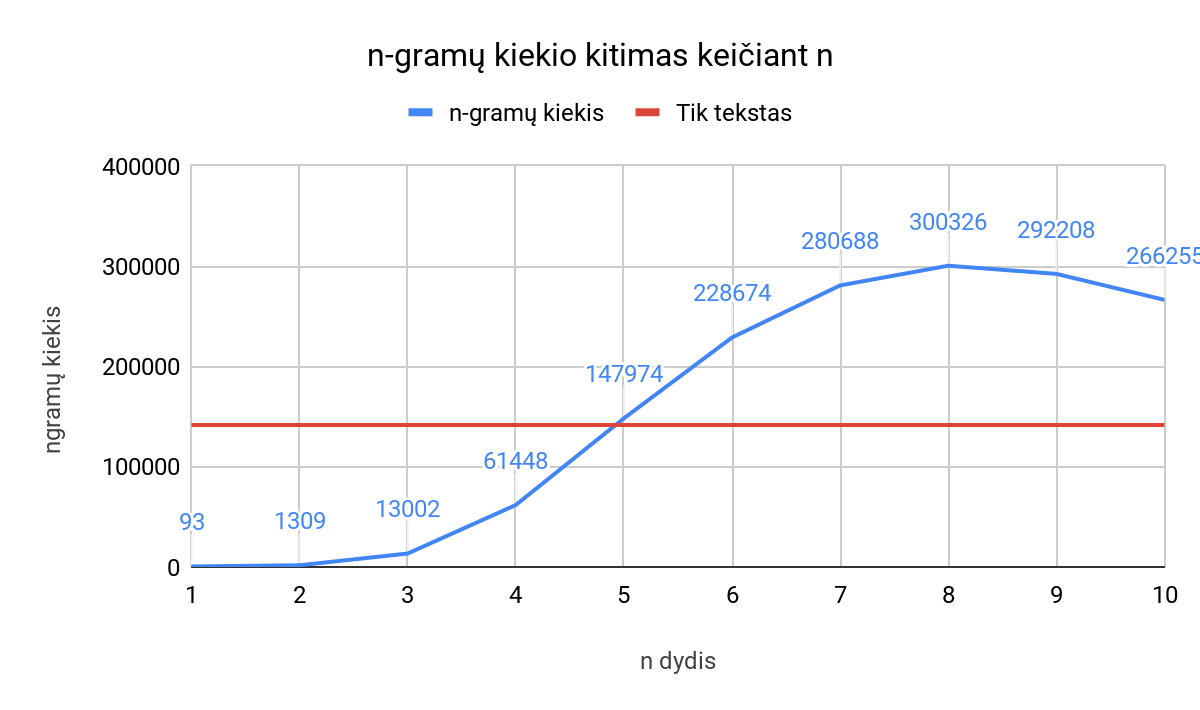
\includegraphics[width=0.8\textwidth]{./img/image7.png}
	\caption{N-gramų (požymių) kiekis su $n$ reikšmėmis nuo 1 iki 10.\\
  Horizontali linija -- tai neapdoroto teksto požymių kiekis. Kai $n$
  = 1, n-gramų net 93 (nors lietuvių kalboje tėra 32 unikalios raidės),
  nes tekstuose yra raidžių iš kitų kalbų abėcėlių.}
  \label{nsize}
\end{figure}

\subsection{Požymių išskyrimas}\label{tfidf}

Norint atlikti tekstinių duomenų analizę su dauguma klasterizavimo
metodų, pirmiausia tekstai turi būti pateikiami skaitine išraiška, todėl
iškyla problema, kaip tinkamai paversti tekstinius duomenis į
skaitinius. Nors yra daugybė požymių išskyrimo (angl. \emph{feature
extraction}) metodų, bet geriausiai naudoti tuos, kurie pritaikyti
duomenims \cite{alelyani2013feature}. Populiariausias tekstiniams duomenims skirtas
metodas yra tf-idf (angl. \emph{term frequency-inverse document
frequency}). Jis yra sudarytas iš dviejų metodų:

\begin{itemize}
\item
  Terminų dažnis (angl. \emph{term frequency}) -- suskaičiuoja kiek
  kartų žodis pasirodė visame dokumentų rinkinyje.
  $$\mathrm{tf} (t,d)=f_{t,d}$$
\item
  Atvirkštinis dokumentų dažnis (angl. \emph{inverse document
  frequency}) -- išmatuoja kiek dažnas yra žodis tarp visų dokumentų.
  Retesniems žodžiams suteikiama didesnė reikšmė.
  $$\mathrm{idf}(t, D) =  \log \frac{N}{|\{d \in D: t \in d\}|}$$
\end{itemize}

Sujungus šiuos metodus gauname:

$${\displaystyle \mathrm {tfidf} (t,d,D)=\mathrm {tf} (t,d)\cdot \mathrm {idf} (t,D)}$$

Iš tf-idf apibrėžimo seka kelios savybės:

\begin{itemize}
\item
  Didžiausi svoriai priskiriami terminams, kurie dažnai pasirodo mažoje
  dokumentų grupėje.
\item
  Daugumoje dokumentų pasirodantys žodžiai turės mažesnius svorius.
\end{itemize}

\begin{figure}[H]
	\centering
	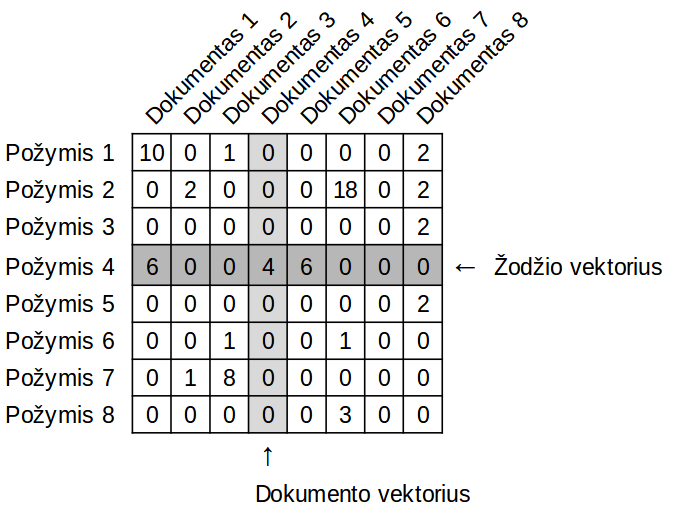
\includegraphics[width=0.65\textwidth]{./img/image25.png}
  \caption{Vektorinės erdvės modelio vizualizacija\\
  Eilutės -- žodžių vektoriai, stulpeliai -- dokumentų vektoriai.\\
  Šaltinis: \cite{marksberry2014employee}}
\end{figure}

\subsection{Klasterizavimo metodai}\label{clustering}

Klasterizavimas tai viena iš neprižiūrimo mokymosi (angl.
\emph{unsupervised learning}) sričių. Jos tikslas -- sugrupuoti duomenis
į klasterius, neturint išankstinės informacijos kaip jie turėtų
atrodyti.

\textbf{Atstumas} -- visų pirma, turime apibrėžti atstumo tarp
  analizuojamų objektų (duomenų) matą. Yra sukurta daugybė skirtingų
  matų ir dažnai jų parinkimas priklauso nuo to, kokius duomenis
  analizuojame. Ankstesniuose žingsniuose tekstiniai duomenys buvo
  paversti į skaitmeninius duomenis, todėl galima panaudoti daugumą
  populiarių matų.

Šiame skyriuje aptarsime keturis, populiarius \cite{wu2008top} ir skirtingai veikiančius, klasterizavimo
metodus\footnote{Klasterizavimo metodai buvo detaliau
  aprašyta kursiniame darbe \url{https://github.com/Kablys/Kursinis/blob/master/kursinis.pdf}}:

\begin{itemize}
\item
  \textbf{K-vidurkių} (angl. \emph{k-means}, toliau -- KV) -- šis
  metodas sukuria $k$ centroidų, kurie atitinka klasterio objektų
  reikšmių vidurkį. Tada iteratyviai vis tikslinama, kurie objektai
  kuriam centroidui turėtų priklausyti ir kokioje padėtyje turėtų būti
  patys centroidai. Kai skirstymas stabilizuojasi, turime sudarytus
  klasterius.
\item
  \textbf{Lūkesčių-maksimizavimo} (angl.
  \emph{expectation--maximization}, toliau -- LM) -- veikimo principas
  labai panašus į KV metodą, tik vietoje centroidų naudojami Gauso
  pasiskirstymai. Dėl to sudaryti klasteriai nėra griežti ir kiekvienas
  objektas priklauso visiems klasteriams su tikimybe.
\item
  \textbf{Hierarchinis} (angl. \emph{hierarchical}) -- skirtingai nei
  ankstesni metodai, šis sugeneruoja ne atskirus klasterius, bet
  klasterių hierarchiją. Dėl to galime duomenyse atrasti kur kas
  sudėtingesnes struktūras. Bet šis metodas reikalauja, kad apibrėžtume
  kaip matuojami atstumai ne tik tarp objektų, bet ir tarp klasterių.
  Trys populiarūs būdai yra šie:

  \begin{itemize}
  \item
    Tolimiausio kaimyno (angl. \emph{furthest neighbor arba complete
    link}) -- atstumas tarp tolimiausių objektų atskiroje poroje
    klasterių.
  \item
    Vidutinių atstumų (angl. \emph{average link}) -- vidutinis atstumas
    tarp visų įmanomų objektų atskiroje poroje klasterių.
  \item
    Ward metodas -- atstumas tarp klasterių centroidų.
  \end{itemize}
\item
  \textbf{DBSCAN} (angl. \emph{density-based spatial clustering of
  applications with noise}) -- metodas kurdamas klasterius, remiasi
  objektų tankiu. Objektai, kurie turi šalia savęs pakankamai kaimyninių
  objektų, virsta klasteriais ir plečiasi kol surenka visus pakankamai
  tankius kaimyninius objektus. Šis metodas sėkmingai ignoruoja
  triukšmą, laikydamas jį nepakankamai tankia zona. Taip pat gali
  sudaryti sudėtingos formos klasterius, vienas klasteris gali net
  pilnai apsupti kitą.
\end{itemize}

Be šių yra dar daugybė skirtingų klasterizavimo metodų ir modifikacijų.
Nėra vieno geriausio universalaus metodo, kiekvienas iš jų turi
privalumų ir trūkumų, todėl reikia parinkti metodą, atsižvelgus į
turimus duomenis ir norimus gauti rezultatus. Buvo atliktas tarpinis
eksperimentas ir nustatyta, kurie iš šių metodų būtų tinkamiausi tekstų
klasterizavimui\footnote{Detaliai šis eksperimentas buvo aprašytas
  kursiniame projektiniame darbe \url{https://github.com/Kablys/Projektinis/blob/master/kursinis.pdf}}.

\subsubsection{Metodų parinkimas}\label{clustest}

Rengiant tekstinių duomenų rinkinį klasterizavimui buvo atlikti šie
žingsniai:

\begin{itemize}
\item
  Panaudoti straipsnių tekstai kaip duomenų šaltinis.
\item
  Atliktas teksto filtravimas: leksinė analizė, naudojant sąrašą
  pašalinti nereikšmingi žodžiai, išgauti žodžių kamienai.
\item
  Išskirti požymiai, panaudojus tf-idf metodą.
\end{itemize}

Atlikus šiuos žingsnius, buvo gauta 4058×47581 dydžio matrica (4058 --
atskiri dokumentai, 47581 -- požymiai). Deja, ši matrica buvo per didelė
porai metodų (LM ir hierarchinio jungiamojo), todėl buvo pasinaudota
„max\_features“ parametru ir palikta pusė požymių (23790).
Klasterizavimas buvo atliktas su „Sci-kit learn“ biblioteka,
klasterizavimo metodams buvo nustatyti šie parametrai:\footnote{Sci-kit
  learn bibliotekoje kiekvienam klasterizavimo metodui yra realizuoti
  skirtingi atstumo matai, todėl buvo nuspręsta palikti numatytas
  atstumo mato parametrų reikšmes.}

\begin{itemize}
\item
  \textbf{K-vidurkių}

  \begin{itemize}
  \item
    \texttt{n\_clusters} -- šis parametras nurodo, kiek klasterių ir tuo
    pačiu kiek centroidų $k$ bus sudaryta. Kadangi straipsniai buvo
    parinkti iš 5 kategorijų, todėl šis parametras taip pat buvo
    nustatytas 5.
  \item
    \texttt{init} -- centroidų inicijavimo metodas. Pasirinktas k-means++.
  \item
    \texttt{n\_init} -- ši KV realizacija lokalaus maksimumo problemą
    sprendžia pakartotinai paleidžiant metodą ir šis parametras nurodo
    kiek kartų tai bus atlikta. Šiuo atveju palikta numatyta reikšmė --
    10.
  \item
    \texttt{max\_iter} -- kiek iteracijų atlikti, palikta numatyta reikšmė
    -- 300.
  \item
    \texttt{random\_state} -- KV veikimui reikalingos atsitiktinės
    reikšmės, todėl norint rezultatus padaryti deterministinius, galima
    nurodyti atsitiktinumo inicializavimo reikšmę (angl. \emph{random
    seed}). Kad rezultatai tarp skirtingų bandymų išliktų stabilūs ir
    nepriklausytų nuo atsitiktinumo, nustatyta inicializavimo reikšmę --
    42.
  \end{itemize}
\item
  \textbf{Lūkesčių-maksimizavimo}

  \begin{itemize}
  \item
    \texttt{n\_components} -- atitinka KV parametrą \emph{n\_clusters}.
  \item
    \texttt{n\_init, max\_iter, random\_state} -- reiškia tą patį kaip ir
    KV parametrai. \texttt{n\_init, max\_iter} buvo paliktos numatytos
    reikšmės, atitinkamai 1 ir 100, \texttt{random\_state} nustatyta --
    42.
  \end{itemize}
\item
  \textbf{Hierarchinis}

  \begin{itemize}
  \item
    \texttt{n\_clusters} -- atitinka KV parametrą.
  \item
    \texttt{linkage} -- nurodo atstumo matavimo / jungimo metodą. „Sci-kit
    learn“ bibliotekos palaikomi: tolimiausio kaimyno, vidutinių atstumų
    ir Ward metodai. Buvo išbandyti visi šie trys metodai.
  \end{itemize}
\end{itemize}

\begin{itemize}
\item
  \textbf{DBSCAN} -- šiam metodui neįmanoma nurodyti grąžinamo klasterių
  skaičiaus, reikia papildomai reguliuoti šiuos parametrus:

  \begin{itemize}
  \item
    \texttt{eps} - maksimalus atstumas iki kaimyno. Buvo išbandytos reikšmės nuo
    0.6 iki 1.3. Mažesnės reikšmės visus duomenis priskirdavo triukšmui,
    didesnės -- visus duomenis priskirdavo vienam klasteriui.
  \item
    \texttt{min\_samples} -- minimalus kaimynų kiekis. Buvo išbandytos reikšmės
    nuo 3 iki 8. Mažesnės reikšmės nėra teoriškai prasmingos naudoti, o
    kuo reikšmė didesnė, tuo klasterių kiekis ir dydžiai mažesni. Be to,
    tyrimo rezultatai parodė, kad išbandyti didesnes reikšmes,
    netikslinga.
  \end{itemize}
\end{itemize}

Klasteriai buvo įvertinti 4 skirtingais būdais, kurie detaliau bus
aptarti \ref{eval} skyriuje. \ref{clusters} diagrama parodo klasterizavimo metodų rezultatus,
įvertintus naudojant išorinius kokybės vertinimo kriterijus.

\begin{figure}[H]
	\centering
	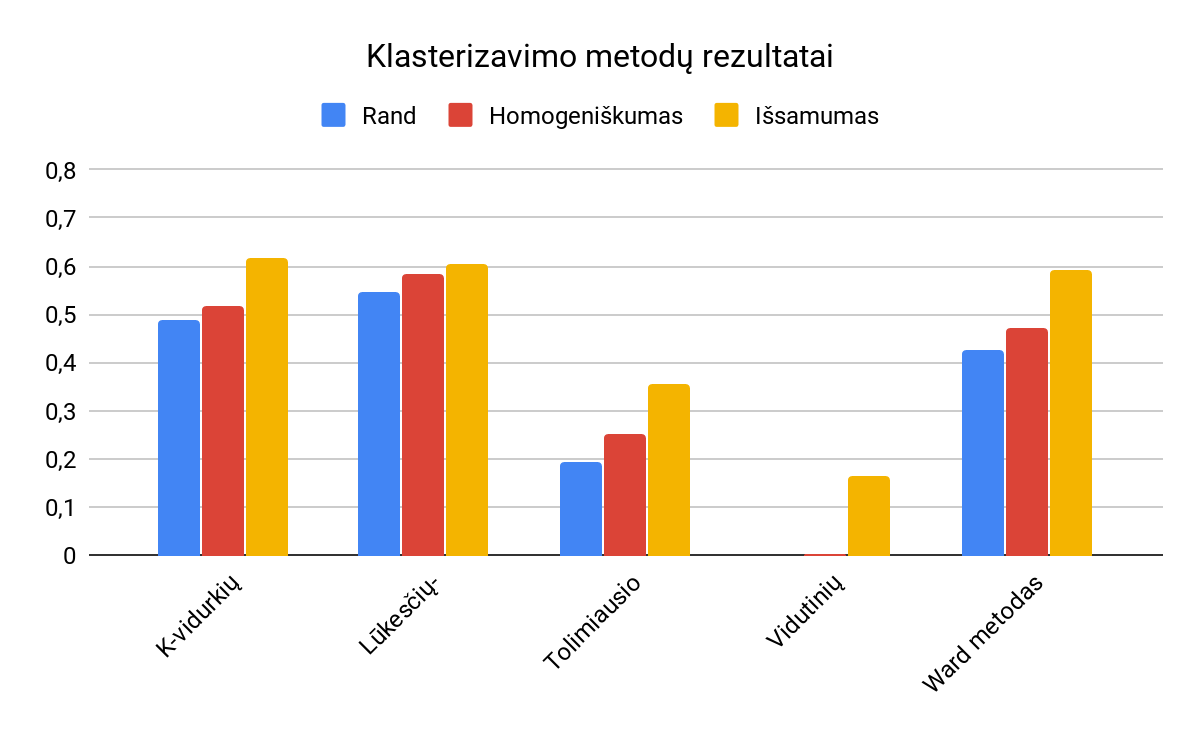
\includegraphics[width=0.8\textwidth]{./img/image27.png}
  \caption{Klasterizavimo metodų rezultatai įvertinti naudojant išorinius
  kriterijus}
  \label{clusters}
\end{figure}

Įvertinus sudarytų klasterių kokybę, buvo išsiaiškinta, kad:

\begin{itemize}
\item
  Mažiausiai tinkamas DBSCAN metodas, nes eksperimento metu buvo gauti
  prasčiausi rezultatai ir reikalavo daugiausia parametrų reguliavimo.
  Nepavyko gauti prasmingo dydžio klasterių be triukšmo, todėl nebuvo
  galima panaudoti išorinio vertinimo kriterijų.
\item
  Praktiškai tokie pat prasti rezultatai gauti naudojant hierarchinį
  vidutinių atstumų metodą.
\item
  Hierarchinis tolimiausio kaimyno metodas pasirodė truputį geriau, bet
  didžioji dalis duomenų pateko į vieną klasterį.
\item
  Ward metodas pateikė pakankamai gerus rezultatus.
\item
  Dėl rezultatų interpretavimo paprastumo ir geros jų kokybės KV ir LM metodai geriausiai tinka lietuviškiems
  tekstiniams duomenims klasterizuoti.
\end{itemize}

Atsižvelgus į tarpinio eksperimento rezultatus, buvo nuspręsta šio darbo
pagrindiniame tyrime naudoti KV, LM ir Ward klasterizavimo
metodus\footnote{Šio tyrimo metu panaudoti visi minėti klasterizavimo
  metodai, bet jie pasirodė taip pat prastai kaip ir tarpiniame
  eksperimente, todėl aptariant šio darbo rezultatus, nebus minimi.} su
tokiais pat parametrais. Buvo panaudoti trys skirtingi metodai, nes šių
klasterizavimo metodų rezultatai yra dalinai priklausomi nuo
atsitiktinumo, todėl norėjosi būti įsitikinus, kad gauti rezultatai nėra
tik atsitiktinumas.

\subsection{Kokybės vertinimas}\label{eval}

Visi klasterizavimo metodai turi bendrą silpnybę -- jų paskirtis atrasti
duomenų struktūras, tačiau jie gali atrasti jas ir tais atvejais, kai
duomenyse nėra jokių struktūrų. Todėl klasterizavimo kokybės įvertinimas
(angl. \emph{evaluation}) yra vienas svarbiausių klasterizavimo proceso
etapų. Jo metu gauti rezultatai parodo ar objektai (duomenys) buvo
teisingai sugrupuoti į klasterius be išankstinės informacijos apie
grupes. Egzistuoja 4 kriterijai klasterizavimo rezultatų kokybei
įvertinti:

\begin{enumerate}
\def\labelenumi{\arabic{enumi}.}
\item
  \textbf{Vidiniai} (angl. \emph{internal}) kriterijai kokybę vertina
  lygindami objektų vienoduose klasteriuose panašumą ir jų skirtumus
  skirtinguose klasteriuose. Deja, šio tipo kriterijai nėra universalūs,
  skirtingiems klasterizavimo metodams reikia parinkti skirtingus
  vidinius kriterijus.
\item
  \textbf{Išoriniai} (angl. \emph{external}) kriterijai kokybę vertina
  lygindami gautus klasterius su jau iš anksto žinomomis duomenų
  klasėmis. Taigi, šiuo atveju vertiname neprižiūrimo mokymosi metodus,
  naudodami prižiūrimam mokymuisi skirtus duomenis. Nors labai tikėtina,
  kad neprižiūrimo mokymosi metodu sugeneruoti rezultatai bus blogesni,
  bet tai vis tiek labai vertingas vertinimo metodas. Tačiau svarbu
  atkreipti dėmesį, kad duomenis dažnai galima sugrupuoti keliais
  skirtingais būdais ir su duomenimis atėjusios etiketės (angl.
  \emph{labels}) nebūtinai yra vienintelis galimas variantas.
\item
  \textbf{Rankiniai} (angl. \emph{manual}) kriterijai, kai kokybė yra
  vertinama žmogaus. Praktikoje tokiu būdu visų sudarytų klasterių
  vertinimas užimtų labai daug laiko. Todėl dažniausiai vertintojui
  duodama pora objektų ir klausiama, ar jie turėtų būti kartu, ar
  atskirai. Surinkę pakankamai rezultatų iš vertintojų, palyginame su
  rezultatais, gautais taikant klasterizavimo algoritmą. Taip pat šiuo
  atveju galima taikyti duomenų vizualizaciją, deja tai tampa ypač
  sudėtinga su didelės apimties duomenimis (tekstiniais dokumentais).
\item
  \textbf{Netiesioginiai} (angl. \emph{indirect}) kriterijai įvertina ar
  klasterizavimas yra vertingas žingsnis, didesnės problemos sprendimui
  (pvz., klasterizavimas naudojamas vaizdų atpažinimui kaip tarpinis
  žingsnis matmenų kiekiui sumažinti). Todėl galime stebėti didesnės
  problemos sprendimo rezultatus su skirtingais klasterizavimo metodais
  (ar jų parametrais) ir parinkti tinkamiausią metodą.
\end{enumerate}

Eksperimente naudosime 3 išorinius kriterijus:

\begin{enumerate}
  \item
    \textbf{Rand indeksas} (toliau Rand) \cite{rand1971objective} – teisingai suklasterizuotų
    objektų dalis:
  
    $$Rand={\frac {TP+TN}{TP+FP+FN+TN}}$$
  
    \begin{table}[h]
      \centering
    \caption{Klasterių kokybės vertinimas}
    \begin{tabular}{|c|c|c|}
    \hline
                & Priklauso klasei                                                                              & Nepriklauso klasei                                                                          \\ \hline
    Priskirtas klasteriui   & \begin{tabular}[c]{@{}c@{}}Teisingai priskirtas\\ (angl. \textit{true positive})\\(TP)\end{tabular}      & \begin{tabular}[c]{@{}c@{}}Neteisingai priskirtas\\ (angl. \textit{false positive})\\(FP)\end{tabular} \\ \hline
    Nepriskirtas klasteriui & \begin{tabular}[c]{@{}c@{}}Neteisingai nepriskirtas\\ (angl. \textit{false negative})\\(FN)\end{tabular} & \begin{tabular}[c]{@{}c@{}}Teisingai nepriskirtas\\ (angl. \textit{true negative})\\(TN)\end{tabular}  \\ \hline
    \end{tabular}
    \label{truefalse}
    \end{table}
  
  \item
    \ltang{\textbf{Homogeniškumas}}{homogeneity} \cite{rosenberg2007v} –
    kiekvienam klasteriui priklauso objektai tik iš vienos klasės:
  
    $$h={1-\frac {H(C|K)}{H(C)}}$$
    $$H(C)=-\sum_{c=1}^{|C|}{\frac {n_c}{n}\cdot\log \left(\frac {n_c}{n}\right)}$$
    $$H(C|K)=-\sum_{c=1}^{|C|}\sum_{k=1}^{|K|}\frac{n_{c,k}}{n}\cdot\log\left(\frac{n_{c,k}}{n_{k}}\right)$$
  
    kur $n$ – bendras objektų kiekis,\\
    $n_c$, $n_k$ – objektų kiekis, priklausantis klasei $c$ ir objektų kiekis priskirtas klasteriui $k$,\\
    $n_{c,k}$ – objektų, priklausančių klasei $c$ ir priskirtų klasteriui $k$, kiekis.
  \item
    \ltang{\textbf{Išsamumas}}{completeness} \cite{rosenberg2007v} -- visi
    klasės objektai priklauso tik vienam klasteriui.
  
    $$c={1-\frac {H(K|C)}{H(K)}}$$
  \end{enumerate}

Specifiniais atvejais homogeniškumo ir išsamumo kriterijai gali gerai
įvertinti blogus klasterius. Pavyzdžiui, suklasterizavimą, kuriame
kiekvienas objektas turi po atskirą klasterį, homogeniškumo kriterijus
įvertins tobulai. Iš kitos pusės, jeigu visi objektai pateks į vieną
klasterį, išsamumo kriterijus jį irgi įvertins tobulai. Nors šie
kriterijai turi trūkumų, bet kartu jie suteikia daug informacijos apie
klasterių savybes.

Be šių kriterijų, tarpiniame eksperimente (žr. sk. \ref{clustest}) rezultatų kokybė dar buvo vertinta ir su keletu
kitų būdų, kuriuos galima būtų laikyti rankiniais kriterijais:

\begin{itemize}
\item
  Sudarytų klasterių dydžiai -- paprasčiausias vertinimo būdas, nes
  kiekvienai kategorijai priklauso panašus kiekis duomenų, todėl vien
  tik stebint sudarytų klasterių dydžius, galima spręsti apie jų kokybę.
  Pavyzdžiui, jeigu didžioji dalis duomenų pateko į vieną klasterį, tai
  galime iš karto nuspręsti, kad rezultatai nebus geri ir nekreipti
  dėmesio į kitus vertinimo metodus. Vertinant DBSCAN metodo rezultatus
  pakako tik šio vertinimo būdo.
\item
  Geriausiai klasterius atitinkančių požymių lentelė (toliau -- požymių
  lentelė). KV ir LM klasterizavimo metodai leidžia paprastai surasti
  klasterių centrus, todėl galime sužinoti, kurie požymiai geriausiai
  atitinka klasterius. Kiekvienam klasteriui buvo atspausdinta po 10
  požymių;
\item
  Sumišimo matrica (angl. \emph{confusion matrix}) -- pavaizduoja kiek
  kurios kategorijos straipsnių pateko į kurį klasterį.
\end{itemize}

Kur buvo prasminga, rezultatai buvo papildomai palyginti, atlikus
klasterių perrikiavimą\footnote{Perrikiavimas veikia taip: kiekvienam
  klasteriui priskiriamas naujas indeksas pagal tai, kuriai kategorijai
  daugiausia jo elementų priklauso. To pasekoje, klasteriai gali būti
  sujungti į vieną (tai ypač svarbu, jei klasterių skaičius būtų
  didesnis nei kategorijų).}. Nors šio darbo tyrime buvo išbandyti visi
vertinimo būdai, darbe nuspręsta pasinaudoti išoriniais kriterijais,
požymių lentelėmis ir papildomai stebėti požymių kiekį.

\section{Eksperimentinio tyrimo rezultatai}

Šiame skyriuje aptarsime tyrime atliktų šešių eksperimentų rezultatus.
Pirmame eksperimente buvo palyginti duomenų šaltiniai, trijuose --
nereikšmingų žodžių pašalinimo metodai, o likusiuose dviejuose --
morfologinės analizės metodai. Nors įprastai atliekant klasterizavimo
tyrimą filtravimo metodai yra kombinuojami, šiuose eksperimentuose jie
bus išbandyti atskirai vienas nuo kito.

Visų tyrimų duomenys buvo suklasterizuoti k-vidurkių,
lūkesčių-maksimizavimo ir Ward metodais. Eksperimentų metu gauti
klasterizavimo rezultatai buvo įvertinti naudojant išorinius kokybės
vertinimo kriterijus\footnote{Šie rezultatai pateikiami stulpelių
  diagramoje. Nors naudojamų išorinių kriterijų galimų reikšmių
  intervalai yra {[}-1; 1{]}, bet diagramos yra nuo 0 iki 0,8, nes į šį
  intervalą pateko visi rezultatai.}, požymių kiekį, požymių
lenteles\footnote{Dėl didelio rezultatų kiekio pagrindiniame tekste
  pateikiamos tik požymių lentelės, kurios aiškiausiai atspindi
  rezultatus, pilnus rezultatus galima rasti \url{https://github.com/Kablys/Bakalaurinio-experiment}}
   ir remtasi asmenine patirtimi\footnote{Vertinant metodų
  realizavimo sudėtingumą, pritaikymą kitose srityse ir kitoms kalboms,
  galimybę kombinuoti su kitais metodais.}, įgyta pasiruošiant ir
atliekant šiuos eksperimentus.

Dalis eksperimentų, pareikalavusių daugiausia operatyviosios atminties
(angl. \emph{RAM}), buvo atlikta naudojantis MIF paskirstytų skaičiavimų
tinklu\footnote{\url{https://mif.vu.lt/cluster/}}.

\subsection{Duomenų šaltinių palyginimas}\label{dsl}

\begin{figure}[H]
	\centering
	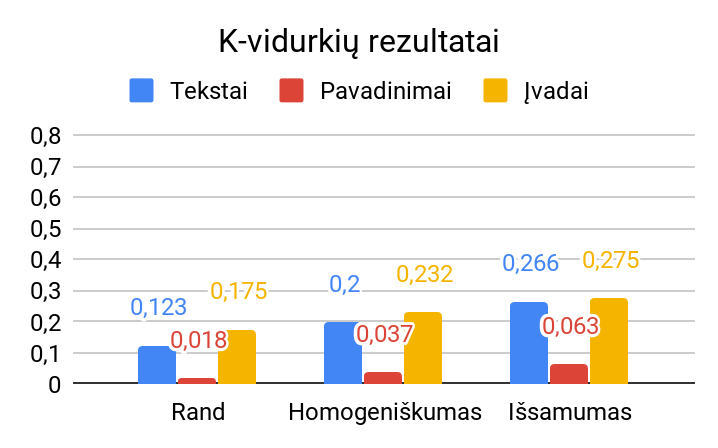
\includegraphics[width=0.6\textwidth]{./img/image21.png}
  \caption{Duomenų šaltinių, suklasterizuotų KV metodu, išoriniai kriterijai}
\end{figure}

\begin{figure}[H]
	\centering
	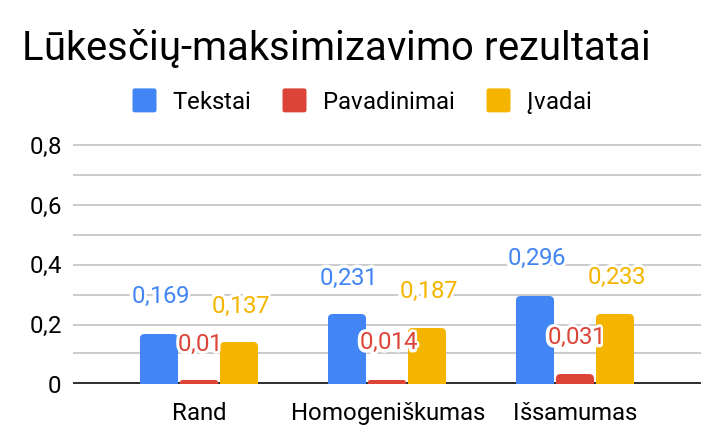
\includegraphics[width=0.6\textwidth]{./img/image2.png}
  \caption{Duomenų šaltinių, suklasterizuotų LM metodu, išoriniai kriterijai}
\end{figure}

\begin{figure}[H]
	\centering
	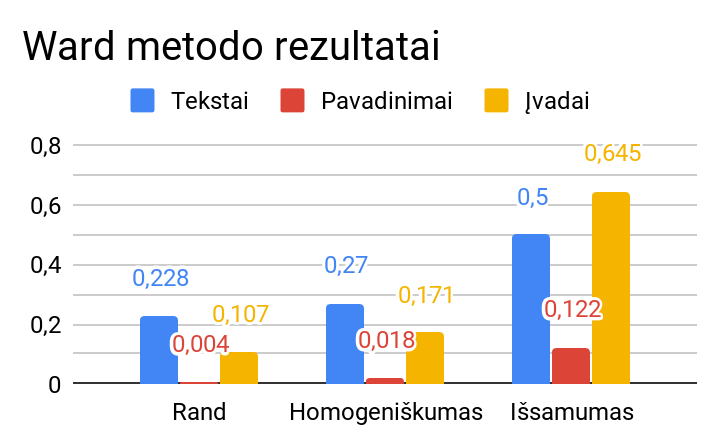
\includegraphics[width=0.6\textwidth]{./img/image10.png}
  \caption{Duomenų šaltinių, suklasterizuotų Ward metodu, išoriniai kriterijai}
\end{figure}

\begin{table}[H]
  \centering
  \caption{Požymių kiekis skirtinguose duomenų šaltiniuose.}
  \begin{tabular}{|l|l|l|l|}
  \hline
  Eksperimentas & Tekstai & Pavadinimai & Įvadai \\ \hline
  Požymių kiekis        & 141331  & 13987       & 32069  \\ \hline
  \end{tabular}
\end{table}

\begin{table}[H]
  \centering
  \caption{Straipsnių tekstų, suklasterizuotų KV metodu, požymių lentelė}
  \small
  \begin{tabular}{|l|l|}
  \hline
  Klasteris 0 & ir min lietuvos po vietą sek su tšk komanda iš  \\ \hline
  Klasteris 1 & ir kad yra su iš buvo tai automobilių ar kaip   \\ \hline
  Klasteris 2 & ir min lietuvos po vietą sek su tšk komanda iš  \\ \hline
  Klasteris 3 & ir kad tai yra su bet ar labai kaip buvo        \\ \hline
  Klasteris 4 & proc ir eurų mln tūkst kad iki jav dolerių metų \\ \hline
  \end{tabular}
  \normalsize
\end{table}

\begin{table}[H]
  \centering
  \caption{Straipsnių pavadinimų, suklasterizuotų KV metodu, požymių lentelė}
  \label{titletable}
  \small
  \begin{tabular}{|l|l|}
  \hline
  Klasteris 0 & automobilių kas naują vokietijos naudotų po ataskaita specialistų kilometrų tūkst \\ \hline
  Klasteris 1 & su kad ir tai apie iš dėl kaip eksperimentą mokslininkai                          \\ \hline
  Klasteris 2 & kaip iš dėl apie lietuvoje ar metų dar už po                                      \\ \hline
  Klasteris 3 & ir apie iš už tik pasaulio savo kaip dėl lietuvoje                                \\ \hline
  Klasteris 4 & lietuvos čempionato rinktinė metų čempionate ir ledo iš europos balso             \\ \hline
  \end{tabular}
  \normalsize
\end{table}

\begin{table}[H]
  \centering
  \caption{Straipsnių įvadų, suklasterizuotų KV metodu, požymių lentelė}
  \small
  \begin{tabular}{|l|l|}
  \hline
  Klasteris 0 & bild auto su kiekvieną sporto žurnalu pastabą smulkiausias ilgalaikiais atliekamais \\ \hline
  Klasteris 1 & ir kad ne ar tik yra gali bet tai tačiau                                            \\ \hline
  Klasteris 2 & lietuvos futbolo čempionato lygos ir pasaulio metų europos čempionate ledo          \\ \hline
  Klasteris 3 & ir automobilių metų nuo eurų lietuvos proc pranešime rašoma žiniasklaidai           \\ \hline
  Klasteris 4 & ir iš savo su buvo lietuvos jau metų po apie                                        \\ \hline
  \end{tabular}
  \normalsize
\end{table}

Pirmame eksperimente buvo išbandyti skirtingi duomenų šaltiniai. Iš
aukščiau pateiktų rezultatų matome, kad straipsnių pavadinimai, kaip
duomenų šaltinis, visuose eksperimentuose pasirodė labai prastai.
Rezultatai buvo beveik tokie pat prasti kaip atsitiktinai parinkus
kuriam klasteriui priklauso dokumentas (atsitiktinis suklasterizavimas
grąžintų Rand, homogeniškumo ir išsamumo reikšmes lygias 0). Vienintelė
išimtis -- išsamumo kriterijaus rezultatai buvo šiek tiek geresni. Kaip
matyti ir iš kitų eksperimentų, išsamumo kriterijus dažnai turėjo
aukščiausias reikšmes, palyginti su kitais kriterijais (ypač kai
naudojamas Ward metodas). Iš to galima teigti, kad skirtingos
kategorijos yra sujungiamos į vieną klasterį\footnote{Taip pat tam
  įtakos turi perrikiavimas, kaip buvo paminėta \ref{eval} skyriuje.}.
Prastus rezultatus taip pat galima įžvelgti ir \ref{titletable} požymių lentelėje, tik klasteris 4 ryškiai sudarytas iš sporto kategorijos
žodžių. Pavadinimai gerai pasirodė tik vienu atžvilgiu -- požymių
kiekiu. Jų straipsnių pavadinimai turėjo net 10 kartų mažiau, nei
straipsnių tekstai. Atlikę šį eksperimentą išsiaiškinome, kad straipsnių
pavadinimai yra netinkamas duomenų šaltinis klasterizavimui. Tam gali
būti daug priežasčių: per mažas požymių kiekis, straipsnių pavadinimais
siekiama skaitytojus sudominti, o ne informuoti.

Tuo tarpu straipsnių įvadų, suklasterizuotų su KV metodu, rezultatai
buvo net geresni, nei klasterizuojant straipsnių tekstus.
Klasterizuojant kitais dviem metodais, rezultatai buvo blogesni. Deja,
iš požymių lentelės vėl buvo galima atskirti tik sporto kategoriją, o
klasterio 1 rezultatus sudarė vien nereikšmingi žodžiai. Tačiau
įvadai turėjo beveik 4,5 karto mažiau požymių, nei straipsnių tekstai.
Visa tai apibendrinus, galima daryti išvadą, kad straipsnių įvadai yra
vertingas duomenų šaltinis klasterizavimui ir verti papildomų
eksperimentų.

Straipsnių tekstai pasirodė geriausiai. Vertinant klasterizavimo
rezultatus su išoriniais kriterijais, dviem iš trijų atvejų, tekstai
pasirodė geriausiai. Požymių lentelėje galima įžvelgti, kad klasteriai
 0 ir 2 yra apie sportą, 1 -- apie automobilius ir 4 yra apie
verslą. Deja, klasteris 3 buvo sudarytas iš nereikšmingų žodžių
(kitoje grupėje eksperimentu bus išbandyti metodai, kurie gali padėti su
tuo susitvarkyti). Tekstai turėjo daugiausia požymių, jų rezultatai buvo
geriausi, todėl buvo laikomi tinkamiausiu šaltiniu ir bus naudojami
kituose eksperimentuose (didelis požymių kiekis net padės, nes leis
lengviau atskirti, kurie metodai sėkmingai mažina požymių kiekį
tekstinių duomenų rinkinyje).

\subsection{Nereikšmingų žodžių pašalinimas}

\subsubsection{Nereikšmingų žodžių sąrašas ir kalbos dalis}\label{stoptest}

\begin{figure}[H]
	\centering
	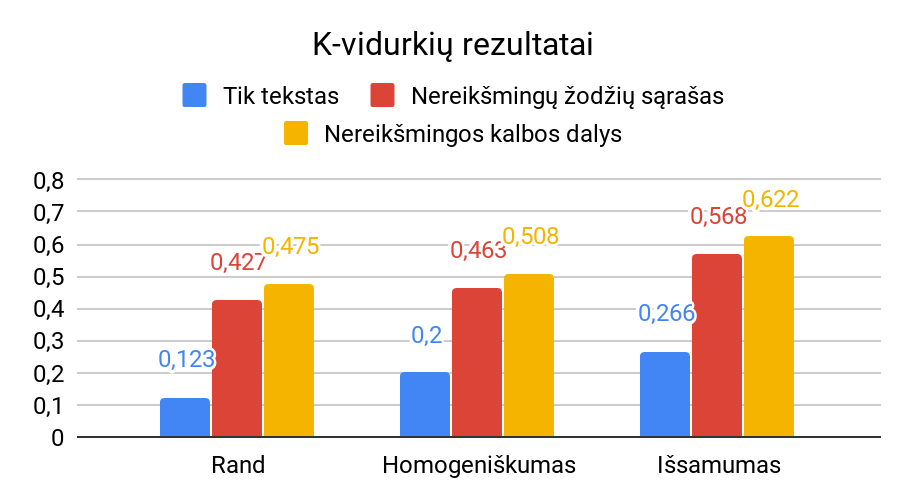
\includegraphics[width=0.6\textwidth]{./img/image15.png}
  \caption{Nereikšmingų žodžių, pašalintų naudojant sąrašą ir kalbos dalis, su KV
  metodu sudarytų klasterių, išoriniai kriterijai}
\end{figure}

\begin{figure}[H]
	\centering
	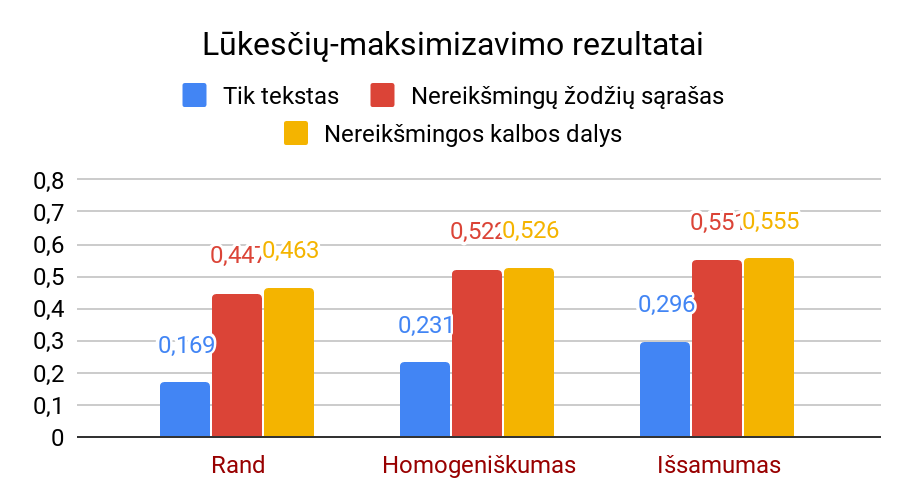
\includegraphics[width=0.6\textwidth]{./img/image12.png}
  \caption{Nereikšmingų žodžių, pašalintų naudojant sąrašą ir kalbos dalis, su LM
  metodu sudarytų klasterių, išoriniai kriterijai}
\end{figure}

\begin{figure}[H]
	\centering
	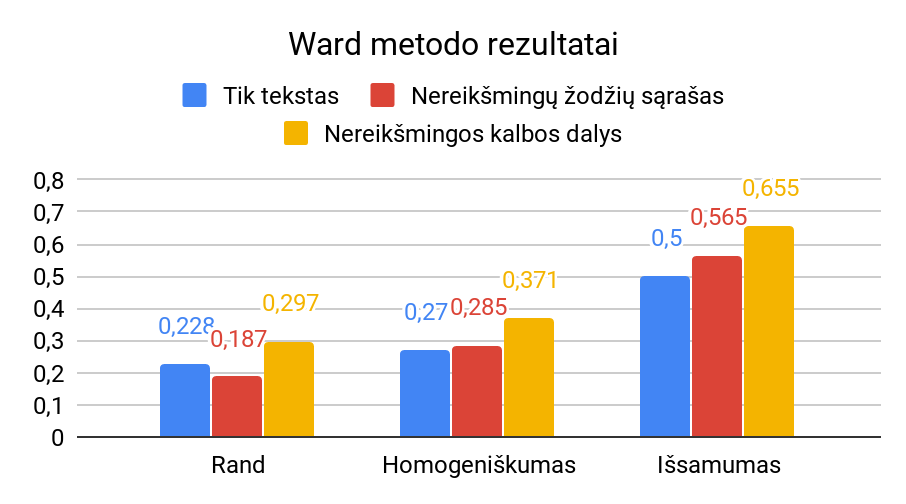
\includegraphics[width=0.6\textwidth]{./img/image19.png}
  \caption{Nereikšmingų žodžių, pašalintų naudojant sąrašą ir kalbos dalis, su Ward
  metodu sudarytų klasterių, išoriniai kriterijai}
\end{figure}

\begin{table}[H]
  \centering
  \caption{Požymių kiekis naudojant skirtingus nereikšmingų žodžių pašalinimo
  metodus}
  \small
  \begin{tabular}{|l|l|l|l|}
  \hline
  Eksperimentas & Tik tekstas & Nereikšmingų žodžių sąrašas & Nereikšmingos kalbos dalys \\ \hline
  Požymių kiekis        & 141331      & 141031                      & 79916                      \\ \hline
  \end{tabular}
  \normalsize
\end{table}

\begin{table}[H]
  \centering
  \caption{Nereikšmingų žodžių, pašalintų naudojant sąrašą, su KV metodu sudarytų
  klasterių, požymių lentelė}
  \label{stoplisttable}
  \small
  \begin{tabular}{|l|l|}
  \hline
  Klasteris 0 & proc eurų mln yra tūkst darbo metų es lietuvos buvo                                 \\ \hline
  Klasteris 1 & yra buvo labai gali jau metų jos jų jie metu                                        \\ \hline
  Klasteris 2 & min rungtynių komanda lygos rungtynes komandos lygoje lietuvos buvo futbolo         \\ \hline
  Klasteris 3 & automobilių eismo transporto automobilio yra iphone automobilis automobilį bus gali \\ \hline
  Klasteris 4 & sporto lietuvos sek pasaulio plaukimo ralio europos buvo vieta lenktynių            \\ \hline
  \end{tabular}
  \normalsize
\end{table}

\begin{table}[H]
  \centering
  \caption{Nereikšmingų žodžių, pašalintų naudojant kalbos dalis, su KV metodu
  sudarytų klasterių, požymių lentelė}
  \label{partstable}
  \small
  \begin{tabular}{|l|l|}
  \hline
  Klasteris 0 & rungtynių komanda lygos rungtynes komandos lygoje taškų minutę lietuvos pelnė             \\ \hline
  Klasteris 1 & sporto lietuvos sek pasaulio buvo ralio lenktynių metų varžybų vieta                      \\ \hline
  Klasteris 2 & yra buvo gali metų metu bus sakė būti metais žmonių                                       \\ \hline
  Klasteris 3 & eurų yra darbo lietuvos metų bus buvo valstybės mokesčių lietuvoje                        \\ \hline
  Klasteris 4 & automobilių eismo transporto automobilio yra automobilis automobilį automobiliai gali bus \\ \hline
  \end{tabular}
  \normalsize
\end{table}

Nereikšmingų žodžių, pašalintų naudojant kalbos dalis, su KV metodu
sudarytų klasterių, požymių lentelė.

Šiame eksperimente buvo palyginti du metodai nereikšmingiems žodžiams
pašalinti -- naudojant nereikšmingų žodžių sąrašą ir nereikšmingas
kalbos dalis. Kaip parodė eksperimento rezultatai, pašalinus
nereikšmingus žodžius naudojant kalbos dalių metodą, išorinių kriterijų
rezultatai buvo šiek tiek geresni, nei naudojant sąrašą. KV ir LM
metodai parodė geresnius rezultatus, pašalinus nereikšmingus žodžius,
nei lyginant su neapdorotais straipsnių tekstais, bet Ward metodas
pasirodė praktiškai taip pat.

Požymių lentelėse taip pat galima matyti geresnius rezultatus -- abiejų
metodų lentelėse galima atpažinti konkrečias temas. Bet jose taip pat
yra akivaizdūs du trūkumai. Pirma, iš \ref{stoplisttable} lentelės klasterio 1 žodžių sunku atpažinti temą ir
daugumą šių žodžių laikytume nevertingais. Šią problemą būtų galima
išspręsti, papildant nereikšmingų žodžių sąrašą. Antra, abiejose
lentelėse galima pastebėti, kad yra daug to pačio žodžio morfologinių
variacijų, tai aiškiausiai matosi \ref{partstable}
lentelės klasteryje 4, kur net 5 iš 10 žodžių prasideda kamienu
„automobil“. Šią problemą padėtų išspręsti morfologinės analizės
metodai.

Požymių kiekio sumažinimas, naudojant kalbos dalis, taip pat pasirodė
geriau -- panaikino 61415 (43,45 \%) požymius, tuo tarpu naudojant
sąrašą (kuris sudarytas iš 485 žodžių.) -- tik 300 (0,21 \%). Iš šio
rezultato galima daryti išvadą, kad nebūtina atlikti didelių pakeitimų
duomenų rinkinyje, kad gauti geresnius rezultatus.

Apibendrinus rezultatus galima teigti, kad, esant galimybei, verta
panaudoti įrankį, kuris gali pašalinti nereikšmingus žodžius pagal
kalbos dalis, bet naudojant sąrašo metodą, galima pasiekti beveik tokių
pat gerų rezultatų.

\subsubsection{Minimalus kiekis}\label{mindftest}

\begin{figure}[H]
	\centering
	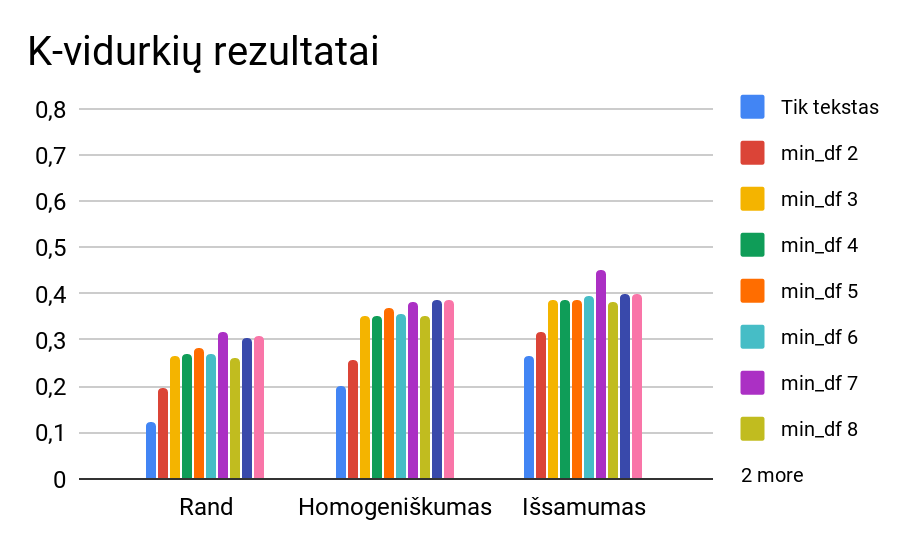
\includegraphics[width=0.6\textwidth]{./img/image11.png}
  \caption{Skirtingų \texttt{min\_df} parametrų, suklasterizuotų KV metodu, išoriniai
  kriterijai}
\end{figure}

\begin{figure}[H]
	\centering
	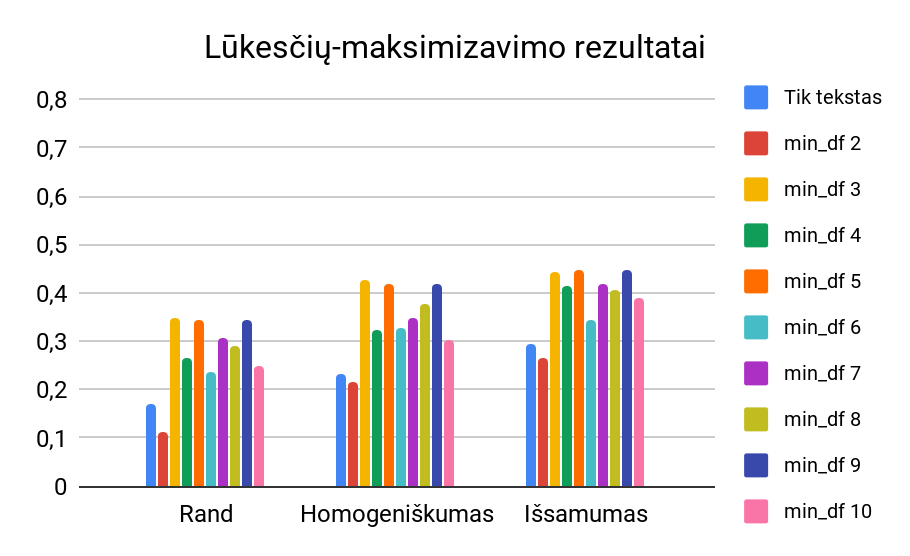
\includegraphics[width=0.6\textwidth]{./img/image18.png}
  \caption{Skirtingų \texttt{min\_df} parametrų, suklasterizuotų KV metodu, išoriniai
  kriterijai}
\end{figure}

\begin{figure}[H]
	\centering
	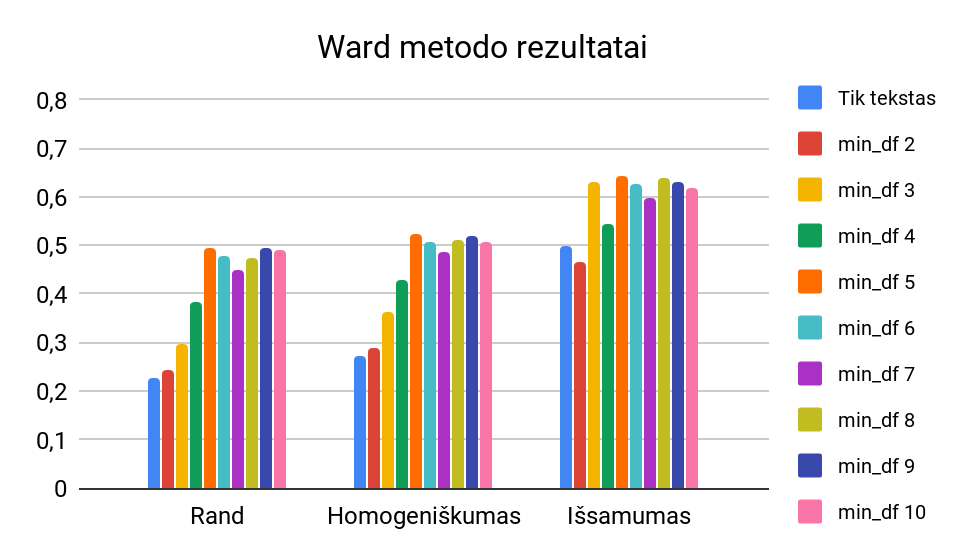
\includegraphics[width=0.6\textwidth]{./img/image23.png}
  \caption{Skirtingų \texttt{min\_df} parametrų, suklasterizuotų KV metodu, išoriniai
  kriterijai}
\end{figure}

\begin{table}[H]
  \centering
  \caption{Požymių kiekis su skirtingais min\_df parametrais}
  \footnotesize
  \begin{tabular}{|l|l|l|l|l|l|l|l|l|l|l|}
  \hline
  Eksperimentas & \multicolumn{1}{c|}{\begin{tabular}[c]{@{}c@{}}Tik \\ tekstas\end{tabular}} & \multicolumn{1}{c|}{\begin{tabular}[c]{@{}c@{}}min\_df\\  2\end{tabular}} & \multicolumn{1}{c|}{\begin{tabular}[c]{@{}c@{}}min\_df\\  3\end{tabular}} & \multicolumn{1}{c|}{\begin{tabular}[c]{@{}c@{}}min\_df\\  4\end{tabular}} & \multicolumn{1}{c|}{\begin{tabular}[c]{@{}c@{}}min\_df\\  5\end{tabular}} & \multicolumn{1}{c|}{\begin{tabular}[c]{@{}c@{}}min\_df\\  6\end{tabular}} & \multicolumn{1}{c|}{\begin{tabular}[c]{@{}c@{}}min\_df\\  7\end{tabular}} & \multicolumn{1}{c|}{\begin{tabular}[c]{@{}c@{}}min\_df\\  8\end{tabular}} & \multicolumn{1}{c|}{\begin{tabular}[c]{@{}c@{}}min\_df\\  9\end{tabular}} & \multicolumn{1}{c|}{\begin{tabular}[c]{@{}c@{}}min\_df\\  10\end{tabular}} \\ \hline
  Požymių kiekis        & 141331                                                                      & 68277                                                                     & 47605                                                                     & 37051                                                                     & 30647                                                                     & 26180                                                                     & 22900                                                                     & 20388                                                                     & 18358                                                                     & 16765                                                                      \\ \hline
  \end{tabular}
  \normalsize
  \end{table}

Šiame ir sekančiame eksperimente išbandėme nereikšmingų žodžių
pašalinimą, pasinaudodami pačio tekstų rinkinio savybe -- žodžių
pasikartojimų dažniais. Šiame eksperimente buvo palyginta, kokią įtaką
klasterizavimo kokybei turi pašalinimas žodžių pagal minimalų jų
pasikartojimo kiekį duomenų rinkinyje (nustatomą parametru
\texttt{min\_df} su reikšmėmis nuo 2 iki 10, neapdorotas tekstas
atitinka reikšmę 1), kitaip tariant, retus žodžius.

Pagal išorinių kriterijų rezultatus galima matyti, kad buvo pagerinti
visų trijų klasterizavimo metodų rezultatai:

\begin{itemize}
\item
  KV metodo rezultatai gerėjo iki \texttt{min\_df} 3 ir tada išsilygino, su
  nežymiu pakilimu \texttt{min\_df} 7. Rezultatai nebuvo tokie geri kaip
  ankstesniame eksperimente, bet vis tiek buvo geresni, palyginti su
  neapdorotu tekstu.
\item
  LM metodo rezultatai buvo nestabilūs. Su \texttt{min\_df} 2 rezultatai buvo
  blogesni nei su neapdorotu tekstu, o su \texttt{min\_df} 3, pasiekė geriausią
  rezultatą ir toliau osciliavo (su lyginiais parametrais rezultatai
  blogesni, su nelyginiais -- geresni), bet išliko geresni nei su
  neapdorotu tekstu.
\item
  Ward metodo rezultatai gerėjo iki \texttt{min\_df} 5 ir tada išsilygino.
  Rezultatai buvo žymiai geresni nei ankstesniame eksperimente, o su
  \texttt{min\_df} 5 Rand rezultatai net viršijo ankstesnio eksperimento
  geriausius rezultatus.
\end{itemize}

Kadangi šis metodas pašalina retai pasitaikančius žodžius, požymių
lentelės nesuteikia vertingų įžvalgų, nes jose matomi dažnai
pasirodantys žodžiai.

Šis būdas taip pat labai efektyvus mažinant požymių kiekį. Su parametru
\texttt{min\_df} 2 požymių kiekis buvo sumažintas daugiau nei perpus (73054
požymiais, 51,69 \%) ir toliau didinant parametrą buvo pašalinamas žymus
požymių kiekis. Pasiekus \texttt{min\_df} 10 teliko 16765 požymiai (11,86 \%).

Apibendrinant galima teigti, kad retai pasitaikančių žodžių pašalinimas
yra vertingas gerinant klasterių kokybę ir sumažinant požymių kiekį.
Taip pat šis metodas lengvai pritaikomas (tinka ne tik tekstiniams
duomenims), realizuojamas ir kombinuojamas su kitais metodais. Verta
atkreipti dėmesį, kad šio parametro reikšmės įtaka rezultatams yra
priklausoma nuo duomenų rinkinio dydžio. Nors šiame eksperimente tokio
atvejo nebuvo, bet galima tikėtis, kad su pakankamai didele
\texttt{min\_df} reikšme, rezultatai gali pradėti blogėti.

\subsubsection{Maksimali dalis}\label{maxdftest}

\begin{figure}[H]
	\centering
	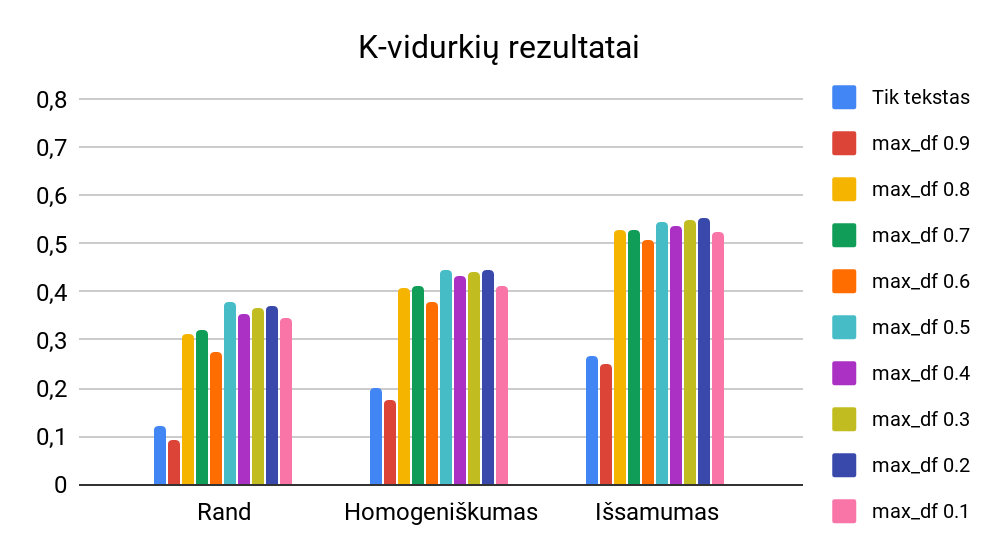
\includegraphics[width=0.6\textwidth]{./img/image26.png}
  \caption{Skirtingų \texttt{max\_df} parametrų, suklasterizuotų KV metodu, išoriniai
  kriterijai.}
\end{figure}

\begin{figure}[H]
	\centering
	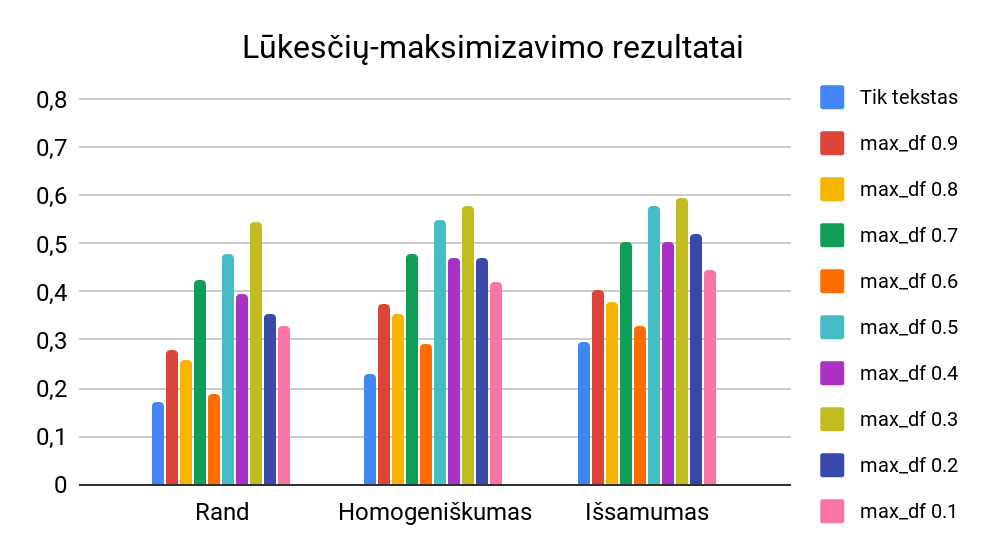
\includegraphics[width=0.6\textwidth]{./img/image3.png}
  \caption{Skirtingų \texttt{max\_df} parametrų, suklasterizuotų LM metodu, išoriniai
  kriterijai.}
\end{figure}

\begin{figure}[H]
	\centering
	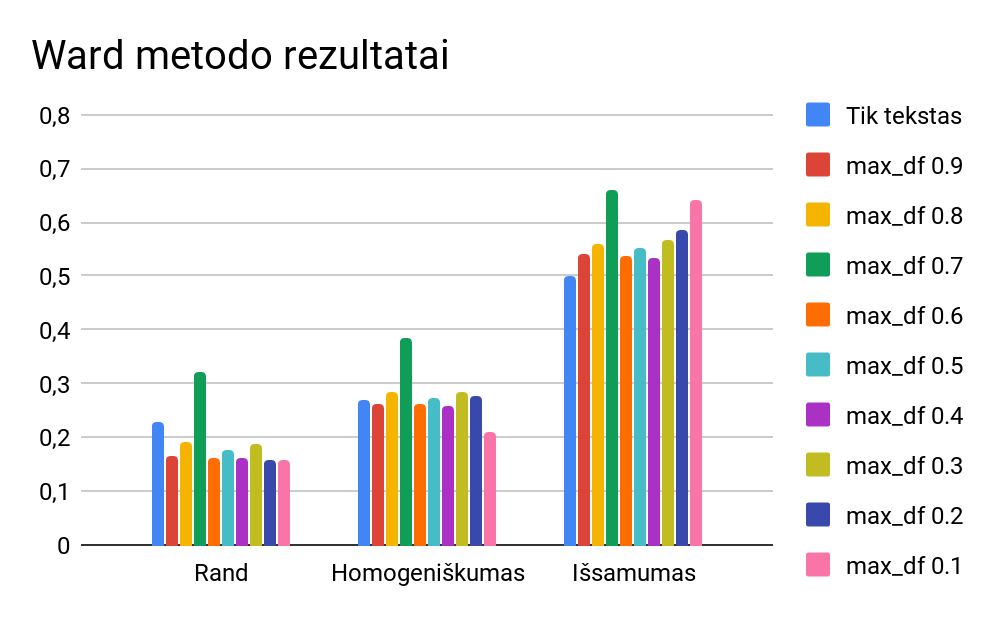
\includegraphics[width=0.6\textwidth]{./img/image4.png}
  \caption{Skirtingų \texttt{max\_df} parametrų, suklasterizuotų Ward metodu, išoriniai
  kriterijai.}
\end{figure}

\begin{table}[H]
  \centering
  \caption{Požymių kiekis su skirtingais \texttt{max\_df} parametrais.}
  \label{maxdfnum}
  \footnotesize
  \begin{tabular}{|l|l|l|l|l|l|l|l|l|l|l|}
  \hline
  \multicolumn{1}{|c|}{Eksperimentas} & \multicolumn{1}{c|}{\begin{tabular}[c]{@{}c@{}}Tik \\ tekstas\end{tabular}} & \multicolumn{1}{c|}{\begin{tabular}[c]{@{}c@{}}max\_df\\  0.9\end{tabular}} & \multicolumn{1}{c|}{\begin{tabular}[c]{@{}c@{}}max\_df\\  0.8\end{tabular}} & \multicolumn{1}{c|}{\begin{tabular}[c]{@{}c@{}}max\_df\\  0.7\end{tabular}} & \multicolumn{1}{c|}{\begin{tabular}[c]{@{}c@{}}max\_df\\  0.6\end{tabular}} & \multicolumn{1}{c|}{\begin{tabular}[c]{@{}c@{}}max\_df\\  0.5\end{tabular}} & \multicolumn{1}{c|}{\begin{tabular}[c]{@{}c@{}}max\_df\\  0.4\end{tabular}} & \multicolumn{1}{c|}{\begin{tabular}[c]{@{}c@{}}max\_df\\  0.3\end{tabular}} & \multicolumn{1}{c|}{\begin{tabular}[c]{@{}c@{}}max\_df\\  0.2\end{tabular}} & \multicolumn{1}{c|}{\begin{tabular}[c]{@{}c@{}}max\_df\\  0.1\end{tabular}} \\ \hline
  Požymių kiekis                              & 141331                                                                      & 141330                                                                      & 141329                                                                      & 141325                                                                      & 141320                                                                      & 141306                                                                      & 141293                                                                      & 141268                                                                      & 141233                                                                      & 141096                                                                      \\ \hline
  \end{tabular}
  \normalsize
\end{table}

\begin{table}[H]
  \centering
  \caption{\texttt{Max\_df} parametrą nustačius 0.1, su KV metodu sudarytų klasterių,
  požymių lentelė}
  \small
  \begin{tabular}{|l|l|}
  \hline
  Klasteris 0 & es valstybės mokesčių prekybos mlrd paslaugų eur įmonių dolerių bendrovės       \\ \hline
  Klasteris 1 & sporto kino mokslininkai muzikos filmo saulės moteris gyvenimo mane pasakojo    \\ \hline
  Klasteris 2 & plaukimo sek krūtine stiliumi meilutytė vieta nugara rapšys laisvuoju peteliške \\ \hline
  Klasteris 3 & eismo iphone automobilis km automobilį automobiliai greičio vairavimo bmw ralio \\ \hline
  Klasteris 4 & min rungtynių lygos rungtynes lygoje tšk minutę rungtynėse taškų rungtynės      \\ \hline
  \end{tabular}
  \normalsize
\end{table}

Šiame eksperimente buvo palyginta, kaip klasterizavimo kokybė yra
įtakojama, pašalinus žodžius pagal maksimalų jų pasikartojimą duomenų
rinkinyje (nustatomą parametru \texttt{max\_df} reikšmėmis nuo 0.9 iki
0.1, neapdorotas tekstas atitinka reikšmę 1.0), kitaip tariant, dažnus
žodžius.

Įvertinę klasterizavimo kokybę išoriniais kriterijais, matome, kad kaip
ir \ref{stoptest}
eksperimente su KV ir LM metodais parengti rezultatai pagerėjo, bet su
Ward metodu -- pablogėjo:

\begin{itemize}
\item
  KV metodo rezultatai su \texttt{max\_df} 0.9 reikšme pablogėjo, bet su 0.8
  reikšme smarkiai pagerėjo, o su likusiomis reikšmėmis, stebima nežymi
  rezultatų gerėjimo tendencija. Bendrai galima pastebėti, kad
  rezultatai pagal kokybę patenka per vidurį tarp anksčiau aprašytų
  dviejų eksperimentų rezultatų.
\item
  LM metodo rezultatai buvo labai nestabilūs. Galima įžvelgti
  tendenciją, kad nuo 0.9 reikšmės kas antras rezultatas vis gerėjo (iš
  šios sekos išsiskyrė blogesniais rezultatais tik 0.1 reikšmė), o nuo
  0.8 -- kas antras rezultatas buvo blogesnis už praėjusį.Tikėtina, kad
  šis nestabilumas kyla dėl to, kad požymių kiekis tarp skirtingų
  parametrų, nežymiai skiriasi (žr. lentelę \ref{maxdfnum}), todėl klasteriai
  sustoja skirtinguose lokaliuose maksimumuose\footnote{Kaip paminėta
    \ref{clustest} skyriuje, LM realizacijoje
    numatytas \emph{n\_init} parametras lygus 1.}.
\item
  Ward metodo rezultatai pasirodė prasčiau, nei neapdorotas tekstas ir
  praktiškai nesikeitė su skirtingomis \texttt{max\_df} reikšmėmis. Vienintelė
  išimtis buvo 0.7 reikšmė. Bendrai galima pastebėti, kad norint gauti
  gerus rezultatus su šiuo metodu, reikia panaikinti ne dažnus o retus
  žodžius.
\end{itemize}

Nors klasterizavimo rezultatai nebuvo tokie geri kaip minimalaus kiekio eksperimente (žr. sk. \ref{mindftest}), bet iš požymių lentelės galima
matyti, kad šis metodas sėkmingai pašalino nereikšmingus žodžius ir
padarė klasterius suprantamesnius. Taip pat matome, kad kaip ir
 nereikšmingų žodžių sąrašo ir kalbos dalių eksperimente (žr. sk. \ref{stoptest}), egzistuoja
daug požymių, kurie tėra to pačio žodžio morfologinės variacijos.

Iš požymių šalinimo pusės, šis metodas labai neefektyvus: 0.9 ir 0.8
reikšmės pašalina tik po vieną požymį, o tarp 1.0 (neapdorotas tekstas)
ir 0.1 buvo pašalinti tik 235 (0,17\%) požymiai (mažiau nei naudojant
nereikšmingų žodžių sąrašą).

Apibendrinus maksimaliai pasikartojančių žodžių kiekio eksperimento
rezultatus, galima teigti, kad šis metodas yra vertingas gerinant
klasterių, parengtų su dalimi klasterizavimo metodų, kokybę, padeda
klasterius padaryti suprantamesnius, bet požymių kiekį sumažina
nereikšmingai. Kaip ir minimalaus kiekio metodas (žr. sk. \ref{mindftest}), šis
metodas lengvai pritaikomas įvairiems duomenims, paprastai realizuojamas
ir kombinuojamas su kitais metodais.

\subsection{Morfologinė analizė}

\subsubsection{Kamienų išgavimas ir lemavimas}

\begin{figure}[H]
	\centering
	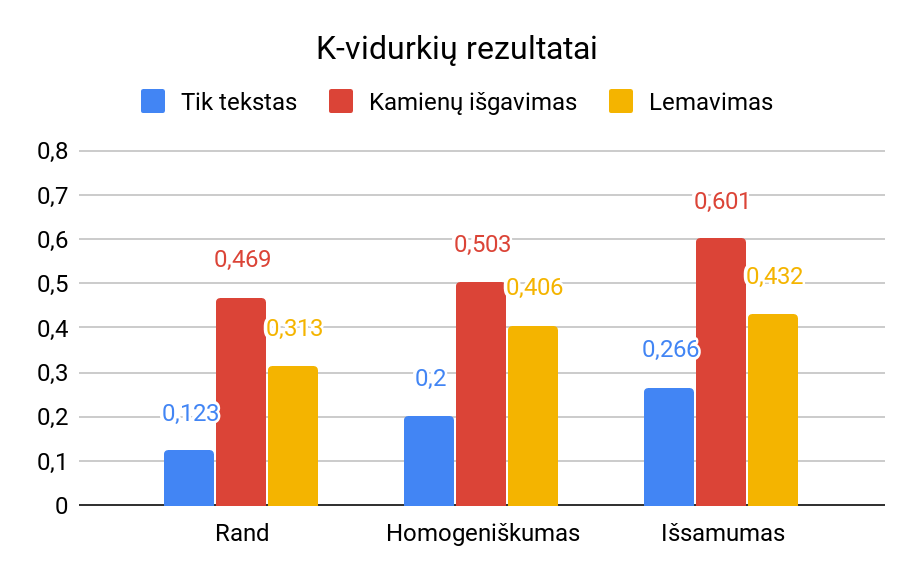
\includegraphics[width=0.6\textwidth]{./img/image14.png}
  \caption{Tekstų kamienų ir lemų, suklasterizuotų su KV metodu, išoriniai
  kriterijai}
\end{figure}

\begin{figure}[H]
	\centering
	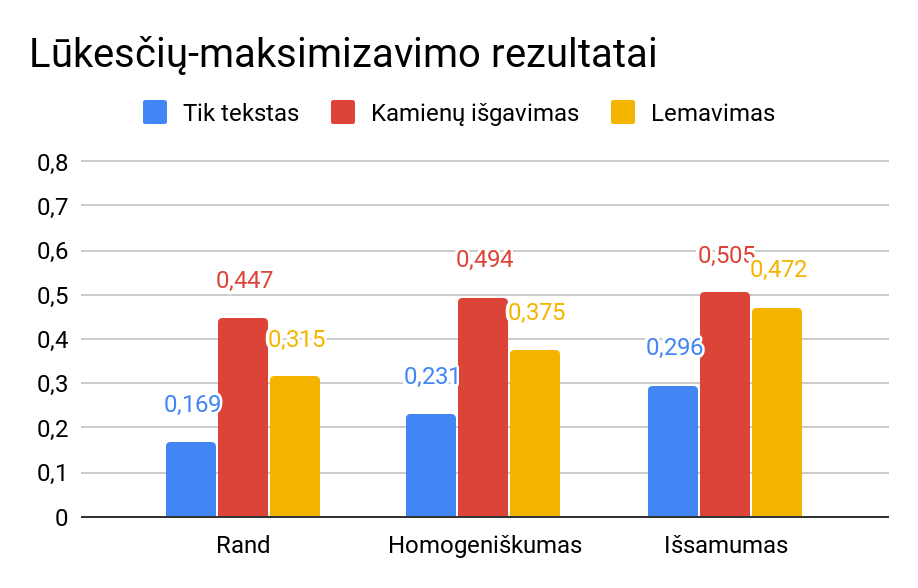
\includegraphics[width=0.6\textwidth]{./img/image17.png}
  \caption{Tekstų kamienų ir lemų, suklasterizuotų su LM metodu, išoriniai
  kriterijai}
\end{figure}

\begin{figure}[H]
	\centering
	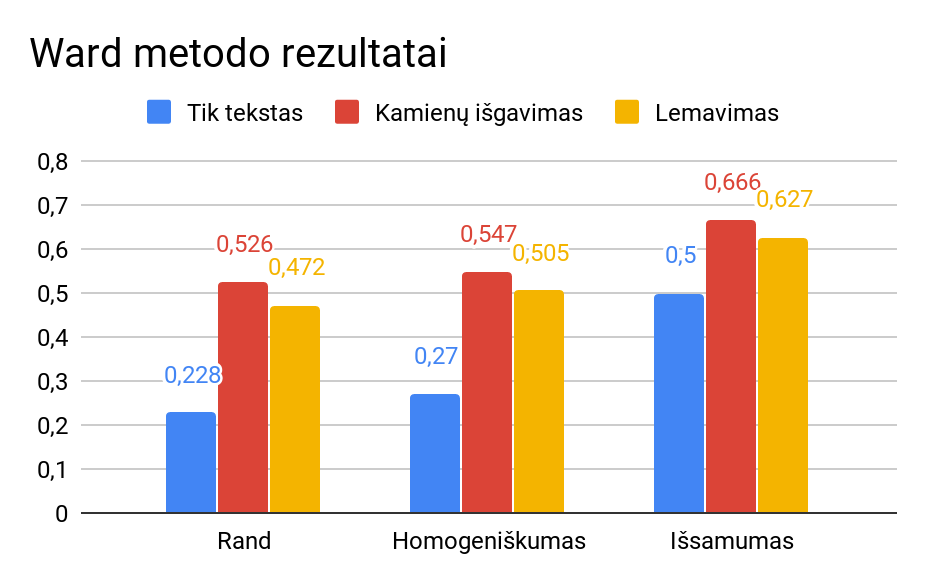
\includegraphics[width=0.6\textwidth]{./img/image16.png}
  \caption{Tekstų kamienų ir lemų, suklasterizuotų su Ward metodu, išoriniai
  kriterijai}
\end{figure}

\begin{table}[H]
  \centering
\caption{Požymių kiekis su skirtingais morfologinės analizės būdais}
\small
\begin{tabular}{|l|l|l|l|}
\hline
Eksperimentas & Tik tekstas & Kamienų išgavimas & Lemavimas \\ \hline
Požymių kiekis        & 141331      & 47668             & 56848  \\  \hline
\end{tabular}
\normalsize
\end{table}

\begin{table}[H]
  \centering
\caption{Tekstų kamienų, suklasterizuotų LM metodu, požymių lentelė}
\small
\begin{tabular}{|l|l|}
\hline
Klasteris 0 & ir kad kur yr met telefon buv gal iš su                     \\ \hline
Klasteris 1 & rungtyn ir komand įvart tašk lietuv žaid pergal lyg čempion \\ \hline
Klasteris 2 & ir eur proc kad met lietuv darb įmon kain mokest            \\ \hline
Klasteris 3 & ir kad man kur tai vis film yr su met                       \\ \hline
Klasteris 4 & automobil ir vair eism kad model transport kel kur gal      \\ \hline
\end{tabular}
\normalsize
\end{table}

\begin{table}[H]
  \centering
\caption{Tekstų lemų, suklasterizuotų LM metodu, požymių lentelė}
\small
\begin{tabular}{|l|l|}
\hline
Klasteris 0 & ir būti jis mokslininkas kad žemė galėti tyrimas šis žmogus                \\ \hline
Klasteris 1 & ir būti jis aš kad tas su kuris žmogus filmas                              \\ \hline
Klasteris 2 & ir būti jis lietuva kad metai šis komanda proc iš                          \\ \hline
Klasteris 3 & automobilis ir būti vairuotojas jis eismas kad transportas kelias modelis  \\ \hline
Klasteris 4 & telefonas iphone išmanus ir programėlė būti apple ekranas įrenginys galėti \\ \hline
\end{tabular}
\normalsize
\end{table}

Šiame eksperimente buvo palyginti du metodai morfologinei analizei
atlikti -- kamienų išgavimo programos (toliau -- stemeris) ir lemavimo
programos (toliau -- lemuoklis) rezultatai. Įvertinę klasterizavimo
rezultatų kokybę išoriniais kriterijais, matome, kad stemeris pasirodė
pastebimai geriau visuose eksperimentuose. Ward metodas aplamai
geriausiai pasirodė iš visų klasterizavimo metodų.

Analizuojant požymių lenteles galima matyti, kad taikant stemerio ir
lemuoklio metodus, sėkmingai iš tekstų pašalintos morfologinės
variacijos, bet išlieka nereikšmingų žodžių problema. Tai ryškiausiai
matoma lemuoklio lentelėje, kur net trijuose klasteriuose trys
populiariausi požymiai yra „ir“, „būti“ ir „jis“. Taip pat iš šių
lentelių galima matyti, kad lemuoklio rezultatai yra lengviau suprantami
ir įskaitomi, nei stemerio.

Analizuojant požymių kiekį galima pastebėti, kad abu metodai pašalino
panašų kiekį požymių, palikdami maždaug trečdalį jų. Vis tik, tarp šių
metodų yra reikšmingas 9180 požymių skirtumas. Viena iš galimų
priežasčių yra ta, kad stermeris yra „agresyvesnis“, nei lemuoklis. Kai
lemuoklis nežino kaip taisyklingai išgauti lemą, palieką žodį
nepakeistą, o stemeris remiasi paprastesnėmis taisyklėmis, todėl gali
dažnai išgauti šaknį, kur jos nėra\footnote{Pavyzdžiui anglišką žodį
  „Apple“ kamienų išgavimo programa grąžins „appl“, o lemuoklis --
  „Apple“.}. Tai galėjo įtakoti geresnius išorinių kriterijų
rezultatus.

Apibendrinant galima teigti, kad abu metodai kokybiškai atlieka
morfologinės variacijos pašalinimą. Kaip matyti iš išorinių kriterijų
rezultatų, stemeris sugeneruoja geresnius klasterius išorinių kriterijų
atžvilgiu, pašalina daugiau požymių ir yra lengviau realizuojamas
(reikalingas kalbos taisyklių failas), bet rezultatai yra sunkiau
įskaitomi ir kombinuojami su kitais metodais, nes yra destruktyvūs.
Lemuoklio klasterizavimo rezultatai yra lengviau įskaitomi ir
kombinuojami su kitais metodais (nes grąžina pilnus žodžius). Tačiau,
kaip matyti iš išorinių kriterijų, lemuoklis sugeneruoja prastesnius
klasterius, pašalina mažiau požymių ir yra sudėtingiau realizuojamas
(reikalinga atskira programa).

\subsubsection{Simbolinės n-gramos}

\begin{figure}[H]
	\centering
	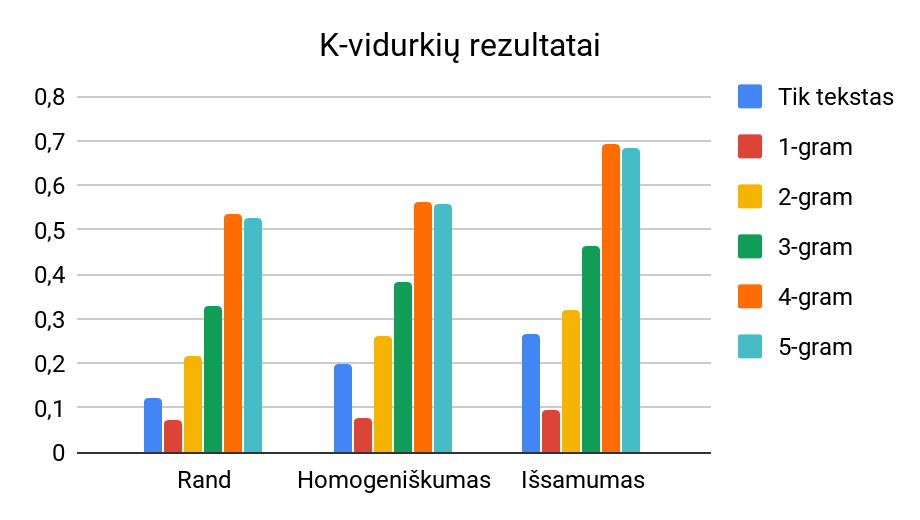
\includegraphics[width=0.6\textwidth]{./img/image8.png}
  \caption{Skirtingų n-gramų dydžių, suklasterizuotų KV metodu, išoriniai
  kriterijai}
\end{figure}

\begin{figure}[H]
	\centering
	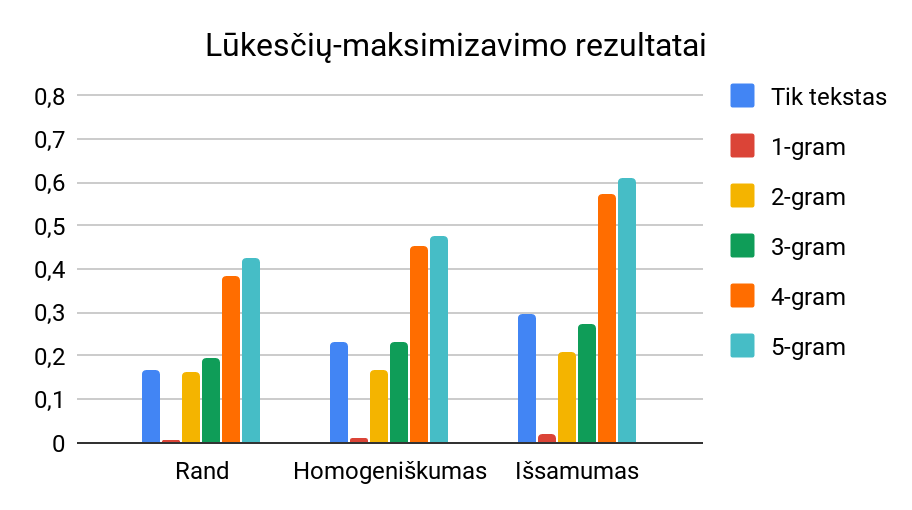
\includegraphics[width=0.6\textwidth]{./img/image24.png}
  \caption{Skirtingų n-gramų dydžių, suklasterizuotų LM metodu, išoriniai
  kriterijai}
\end{figure}

\begin{figure}[H]
	\centering
	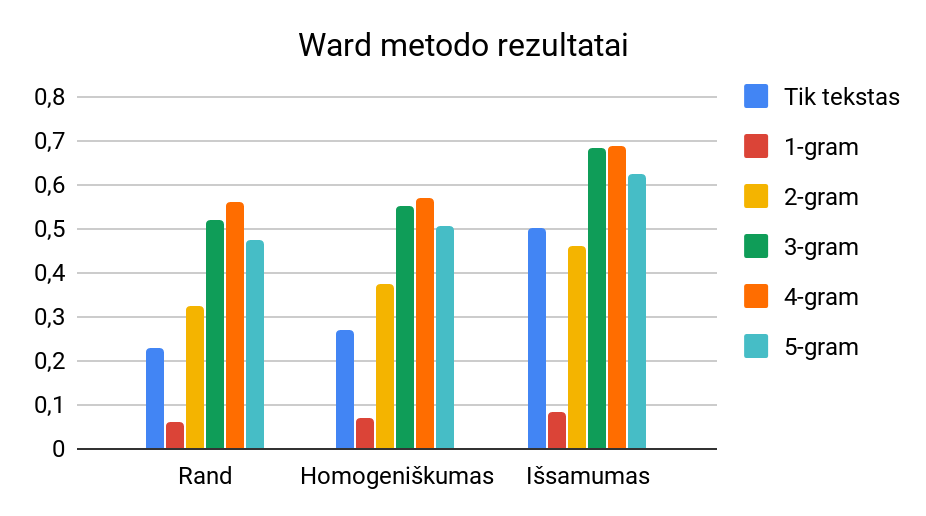
\includegraphics[width=0.6\textwidth]{./img/image20.png}
  \caption{Skirtingų n-gramų dydžių, suklasterizuotų Ward metodu, išoriniai
  kriterijai}
\end{figure}

\begin{table}[H]
  \centering
  \caption{Tekstų 3-gramų, suklasterizuotų LM metodu, požymių lentelė}
  \small
  \begin{tabular}{|l|l|}
  \hline
  Klasteris 0 & sn sni ai os is ėžo šl ieg ke kel \\ \hline
  Klasteris 1 & pa ai as os ti is ka us pr ne     \\ \hline
  Klasteris 2 & os pa as ai is pr us ių ka ti     \\ \hline
  Klasteris 3 & as ai pa ka os is ti us ir ir     \\ \hline
  Klasteris 4 & as os pa ai is us ir ir je ka     \\ \hline
  \end{tabular}
  \normalsize
\end{table}

\begin{table}[H]
  \centering
  \caption{Tekstų 4-gramų, suklasterizuotų LM metodu, požymių lentelė}
  \small
  \begin{tabular}{|l|l|}
  \hline
  Klasteris 0 & ir oksl moks kad mok slin kad ksli gal kosm    \\ \hline
  Klasteris 1 & ir pas kad kad pri tai pro iau kur iai         \\ \hline
  Klasteris 2 & ir spo spor port čemp mpio pion empi ktyn nkty \\ \hline
  Klasteris 3 & omob mobi obil utom aut auto tomo ir bili pri  \\ \hline
  Klasteris 4 & gtyn ngty run rung ungt ir oman mand žai žaid  \\ \hline
  \end{tabular}
  \normalsize
\end{table}

Paskutiniame eksperimente išbandytos simbolinės n-gramos, kaip
paprastesnė morfologinės analizės alternatyva stemeriams ir lemuokliams.
Kaip matome iš pateiktų rezultatų, pagal išorinius kriterijus n-gramos
pasirodė gerai su visais trimis klasterizavimo metodais. 1-gramos
pasirodė žymiai prasčiau, nei neapdorotas tekstas, bet to buvo galima
tikėtis, nes šiuo atveju požymiai sudaryti tik iš atskirų raidžių.
Tekstą suskaidžius į simbolines 2-gramas, LM metodu sudarytų klasterių
rezultatai buvo tokie pat geri, kaip ir su neapdorotu tekstu, o
rezultatai parengti KV ir Ward metodais, net geresni. Toliau suskaidžius
tekstą 3-gramomis, rezultatai gerėjo, kol išsilygino ties 4-gramomis
(viršydami ankstesnio eksperimento KV ir Ward rezultatus) kaip ir su
kitomis europinėmis kalbomis.% (žr. sk. \ref{ngram}).

Iš požymių lentelių galime pastebėti, kodėl rezultatų gerėjimas sustoja
ties 4-gramomis. Iš 3-gramų vis dar sunku atpažinti žodžius ar atskiras
kategorijas, bet su 4-gramomis jau galima atpažinti žodžius, pavyzdžiui,
„moks“, „rung“, „auto“\footnote{Vidutinis stemerio sugeneruoto
  požymio ilgis yra 4,69 (vidutinis žodžio ilgis 6,33, lemos -- 6,24),
  iš to galime spėti, kad galbūt n-gramos gali dalinai išgauti kamienus.}.

Iš anksčiau pateikto grafiko \ref{nsize} galima
matyti, kad su mažomis $n$ reikšmėmis n-gramos yra efektyvus
metodas sumažinti požymių kiekį, bet su didesnėmis $n$ reikšmėmis,
požymių kiekis gali labai smarkiai išaugti (šių duomenų atveju net
viršyti neapdoroto teksto požymių kiekį).

Apibendrinant galima teigti, kad parinkus tinkamą $n$
reikšmę, n-gramos gali parengti panašios kokybės klasterizavimo
rezultatus kaip stermeriai ir lemuokliai, smarkiai sumažinti požymių
kiekį ir yra lengvai realizuojamos. Bet n-gramų rezultatai yra sunkiau
įskaitomi (iš raidžių sekos sunkiau atpažinti žodį nei iš šaknies),
požymių kiekis gali staiga netikėtai išaugti.

\sectionnonum{Išvados}
Šiame darbe buvo pasiektas užsibrėžtas tikslas -- palyginti skirtingi
tekstinių duomenų parengimo klasterizavimui metodai ir nustatyta, kurie
iš jų geriausiai tinka lietuviškiems tekstiniams dokumentams.

Siekiant užsibrėžto tikslo buvo atlikti šie darbai:

\begin{itemize}
\item
  Sudarytas didelės apimties lietuviškų tekstinių duomenų rinkinys iš
  5-ių skirtingų kategorijų ir 4058 skirtingų straipsnių. Kaip galimi
  klasterizavimo duomenų šaltiniai, eksperimentų metu buvo palyginti
  straipsnių pavadinimai, įvadai ir tekstai.
\item
  Rengiant tekstinių duomenų rinkinius klasterizavimui pritaikyta
  leksikos analizė ir eksperimentuose buvo palyginti tekstinių duomenų
  filtravimo metodai:

  \begin{itemize}
  \item
    Nereikšmingų žodžių pašalinimas: su nereikšmingų žodžių sąrašu,
    pašalinant nereikšmingas kalbos dalis ir pagal tai kaip dažnai žodžiai pasikartoja
    duomenų rinkinyje.
  \item
    Morfologinė analizė: atskiriant žodžių kamienus, išgaunant žodžių
    lemas, suskaidant žodžius į n-gramas.
  \end{itemize}
\item
  Skaitinių požymių išskyrimui iš tekstų buvo panaudotas tf-idf metodas.
\item
  Apžvelgti ir išbandyti šeši klasterizavimo metodai ir nuspręsta, kad
  eksperimentuose naudoti: k-vidurkių, lūkesčių-maksimizavimo,
  hierarchinio jungiamojo su Ward atstumo matavimo / jungimo metodus.
\item
  Klasterizavimo rezultatų kokybė buvo vertinama išoriniais kriterijais: Rand
  indeksu, homogeniškumu ir išsamumu. Taip pat eksperimentų rezultatams
  vertinti naudotas požymių kiekis ir požymių lentelės.
\end{itemize}

Kaip parodė eksperimentų rezultatai:

\begin{itemize}
\item
  Klasterizavimui tinkamiausias duomenų šaltinis yra straipsnių tekstai,
  kiek prasčiau tinka įvadai ir visai netinkami straipsnių pavadinimai.
\item
  Nereikšmingų žodžių pašalinimas naudojant kalbos dalis, grąžina šiek
  tiek geresnius rezultatus, nei nereikšmingų žodžių sąrašas. Tačiau
  žodžių sąrašas yra kur kas paprastesnis metodas. Taikant minimalaus kiekio
  metodą šiek tiek pagerėjo eksperimento rezultatai, bet buvo pašalintas didžiausias požymių
  kiekis palyginti su kitais metodais. Maksimalios dalies metodo rezultatai
  irgi buvo geri ir lengvai įskaitomi. Šie du metodai lengvai pritaikomi
  įvairiems duomenims ir kombinuojami su kitais metodais.
\item
  Atliekant morfologinę analizę kamienų išgavimo metodas sugrąžino
  geresnius rezultatus, nei lemavimo metodas. Be to, kamienų išgavimo
  metodas lengviau realizuojamas, bet lemuoklio rezultatai yra lengviau
  įskaitomi. N-gramos grąžino geriausius rezultatus ir yra labai
  paprastai realizuojamos. Kaip parodė tyrimo rezultatai, lietuviškiems
  tekstams tinkamiausios yra 4-gramos. Deja, bet n-gramų rezultatai yra
  sunkiausiai įskaitomi ir kombinuojami su kitais metodais.
\end{itemize}

Apibendrinus eksperimentų rezultatus galima teigti, kad geriausias
duomenų šaltinis yra straipsnių tekstai, geriausias būdas pašalinti
nereikšmingus žodžius -- naudoti kalbos dalis, geriausias būdas atlikti
morfologinę analizę -- naudoti 4-gramas. Tačiau visi apžvelgti metodai
yra vertingi ir pasirinkimas priklauso nuo to kas svarbiau: klasterių
kokybė, rezultatų suprantamumas ar realizavimo sudėtingumas.

\paragraph{Galimos tolimesnės tyrimų sritys}

Atliekant eksperimentus buvo pastebėta keletas sričių, kurias verta
detaliau patyrinėti:

\begin{itemize}
\item
  Išbandyti skirtingų metodų kombinacijas. Prasmingiausia būtų pabandyti
  sujungti nereikšmingų žodžių metodą su morfologine analize.
\item
  Paeksperimentuoti su skirtingais klasterizavimo metodų parametrais.
\item
  Kadangi straipsnių įvadai, kaip duomenų šaltinis, parodė neblogus
  rezultatus, būtų vertinga išbandyti juos kaip pagrindinį šaltinį arba
  pabandyti sujungti su straipsnių tekstais.
\item
  Leksikos analizės etape pabandyti palikti tekste skaičius (ar kitus
  simbolius).
\item
  Išbandyti nuo kokios \texttt{min\_df} ir \texttt{max\_df} parametrų reikšmės rezultatai
  pradeda blogėti ir kaip jie yra priklausomi nuo dokumentų skaičiaus.
\item
  Pakartoti maksimalios dalies (žr. sk. \ref{maxdftest}) eksperimentą su LM
  algoritmu, bet su didesnėmis \texttt{n\_init} reikšmėmis.
\end{itemize}

Atliekant šį darbą buvo susidurta su šalutinėmis temomis, kurios buvo
nesusijusios su iškeltais uždaviniais, bet vertos patyrinėti ir
įvertinti su lietuviškais tekstais.

\begin{itemize}
\item
  Išbandyti kitus klasterizavimo metodus:

  \begin{itemize}
  \item
    \textbf{Tinkleliu} (angl. \emph{grid}) pagrįstus metodus \cite{mivm2010}.
  \item
    Klasterizavimą Kohonen \textbf{neuroniniu tinklu} (angl.
    \emph{Kohonen net clustering)} \cite{kohonen2007kohonen}.
  \item
    \textbf{Genetiniais} algoritmais grindžiamus klasterizavimo
    algoritmus (angl. \emph{genetically guided algorithm}) \cite{hall1999clustering}.
  \end{itemize}
\item
  Klasterių žymėjimas (angl. \emph{Cluster labeling}) -- metodas,
  skirtus surasti žodžius, geriausiai apibendrinančius klasteryje
  esančius dokumentus.
%\item Erdvių sumažinimo (angl. \emph{Dimensionality reduction}) metodai.
%\item Temų modeliavimas (angl. \emph{Topic modeling}) -- metodas, skirtas tekstiniuose duomenyse rasti temas.
\item
  Dokumentų klasifikavimas (angl. \emph{Document Classification}) --
  prižiūrimo mokymosi sritis, kur dokumentą bandoma priskirti vienai iš
  kelių, iš anksto žinomų klasių.
\end{itemize}

\sectionnonum{Conclusions}

With ever-increasing amount of data being produced it is becoming more
and more relevant to find a better ways of searching, organizing and
making insights into data. Work with a big amounts of text data could be
improved by using document clustering methods. However, to get good
clustering results it is important to properly prepare a data sets for
clustering. There are a lot of methods for filtering text data and
sometimes it is not clear which ones are best for the task at hand. So the
main objective of this work was: to evaluate different ways of preparing text
data for clustering and find out which of them works best for Lithuanian language
text.

To accomplish the main objective, all relevant topics for document clustering
were addressed. Extracting data set from a Lithuanian news website.
Lexical analysis to break text into a series of words. Three ways to
remove unnecessary word (stop-words) from a text: stop-word lists, parts
of speech, frequency of word in the data set. Three ways of combining
similar words into one: extracting word stems from words, turning word
into its lemma (dictionary form), split words into n-grams. Numerical
feature extraction from the text data using tf-idf. Overview of different
types of clustering methods. Types and examples of cluster evaluation.

In conclusion for best clustering results: as a source of a data article
texts were best, for removing stop-words it is best to remove parts of
speech, for morphological analysis 4-grams are the best. However, all
evaluated methods, had advantages and drawbacks depending what is the
goal: the best possible clustering, intelligible results or difficulty
of implementation.

\printbibliography[heading=bibintoc] % literatūros šaltiniai aprašomi
% bibliografija.bib faile. šaltinių sąraše nurodoma panaudota literatūra,
% kitokie šaltiniai. abėcėlės tvarka išdėstoma tik darbe panaudotų (cituotų,
% perfrazuotų ar bent paminėtų) mokslo leidinių, kitokių publikacijų
% bibliografiniai aprašai (šiuo punktu pasirūpina latex). aprašai pateikiami
% netransliteruoti.

\appendix  % Priedai
% Prieduose gali būti pateikiama pagalbinė, ypač darbo autoriaus savarankiškai
% parengta, medžiaga. Savarankiški priedai gali būti pateikiami kompiuterio
% diskelyje ar kompaktiniame diske. Priedai taip pat vadinami ir numeruojami.
% Tekstas su priedais siejamas nuorodomis (pvz.: \ref{img:mlp}).

\end{document}
